\chapter{Control System Implementation}
\label{implementation_of_controller}

This chapter explains how the controller designed in \chapref{Controller} is desired to be implemented on the scaled system at Aalborg university.  

\section{Simulink implementation}
\label{simulink_intro}
In the implementation of the control, the model estimated in \secref{estim_results} is used. Although the fit percentage differs from the real data, the behavior and dynamics of the WT are qualitatively correct, making this model the most suitable and realistic one to work with. \figref{fig:control_sketch} shows the implementation strategy for the control design on the model of the water distribution system.
% It is worth mentioning, that for the implementation of the control, the second linear model attempt is used as it is the most suitable model to work with. The MPC controller is implemented in MATLAB Simulink, which is connected to the model as shown in \figref{fig:control_sketch}:

\begin{figure}[H]
\centering
\begin{tikzpicture} [scale=0.67,transform shape]

\draw  (10,2) rectangle (6,0);
\node at (8,1) {Model};
\node at (9.7,1.7) {y};
\node at (9.7, 0.3) {x};
\node at (6.3, 1.7) {d};
\node at (6.3, 0.3) {u};
\draw[-triangle 60] (10, 1.7) -- (11, 1.7);

\draw[-triangle 60] (10, 0.3) -- (11, 0.3) -- (11,-3) -- (9,-3);



\draw  (9,-2) rectangle (7,-4);
\node at (8,-3) {MPC};
\node at (6.5,-2.55) {$\bm{U_{Hp}}$};
\draw  (7,-3) -- (6,-3);
\draw (6,-3.3) rectangle (4,-2.7);
\draw (8.3,-2) rectangle (7.7,-2.5);
\node at (8, -2.2) {$T_s$};

\draw  (5.8,-3.3) -- (5.8,-2.7);
\draw  (5.6,-3.3) -- (5.6,-2.7);
\draw  (5.4,-3.3) -- (5.4,-2.7);
\draw  (5.2,-3.3) -- (5.2,-2.7);
\draw  (5.0,-3.3) -- (5.0,-2.7);
\draw  (4.8,-3.3) -- (4.8,-2.7);
\draw  (4.6,-3.3) -- (4.6,-2.7);
\draw  (4.4,-3.3) -- (4.4,-2.7);
\draw  (4.2,-3.3) -- (4.2,-2.7);
\fill[ForestGreen] (4.18,-3.29) rectangle(4.01,-2.71);
\draw[-triangle 60] (4, -3) -- (3, -3) -- (3,0.3) -- (6,0.3);
\node at (3.9,-1.5) {$\bm{U_{Hp}}(1,1)$};
\draw[-triangle 60] (5,1.7)--(6,1.7);

 
 	\draw (0,1.7) -- (4.3,1.7);
 	\node [font=\tiny] at (4.3,1.5) {t};
    \draw (0,2.4)node[left,font=\tiny] {$OD$} -- (0,1.0);
    % \draw (0.2,-1)node[left,font=\tiny] {$y=-1$} -- (11.8,-1); 
    % \foreach \x in {0,0.5,...,12}{
    % \draw (\x,-0.2)node [below,font=\tiny,] {\x} -- (\x,0.2) ;
    % }
    \draw[ thick, red] (0,1.7) sin (0.7,2.4);    %% the real business in this line
    \draw[ thick, red] (0.7,2.4) cos (1.4,1.7);    %% the real business in this line
    \draw[ thick, red] (1.4,1.7) sin (2.1,0.9);    %% the real business in this line
    \draw[ thick, red] (2.1,0.9) cos (2.8,1.7);    %% the real business in this line
    \draw[ thick, red] (2.8,1.7)  sin (3.5,2.4);    %% the real business in this line
    \draw[ thick, red] (3.5,2.4) cos (4.2,1.7);    %% the real business in this line
    % \draw[ultra thick, red] (9,0) sin (10,-1);    %% the real business in this line
    % \draw[ultra thick, blue] (10,-1) cos (11,0);    %% the real business in this line

\end{tikzpicture}%


 
\caption{Sketch of the control implementation.}
\label{fig:control_sketch}
\end{figure}

In the block diagram, the state-space box represents the estimated plant with inputs defined by the control, $u$, and disturbance signals, $d$. The output of the state-space model is the pressure around the end-user valves, $y$. In Simulink, the state of the system, i.e. the WT pressure is also defined as an output. As the current value of the initial state is measured, it is sent to the MPC block at each iteration step. This iteration step is defined by the sampling time, $T_s$ of the MPC block which runs the minimization algorithm at each of this time steps. When the algorithm is done, the control signal for the prediction horizon is saved as $\bm{u_{Hp}}$. Although the prediction is calculated for the future price scenarios, only the first element in $\bm{u_{Hp}}$ is picked for control. After applying the first entry of $\bm{u_{Hp}}$, the iteration continues with the next time step. In the next step the price and disturbance sequences are shifted one time step further and then a new measurement is carried out on the model again.

In order to solve the optimization and find a global minimum for the problem specified in \eqref{eq:obj_final1},  Quadratic Programming(QP) is used. Solvers for QP problems in Matlab are well developed and available in a wide range, therefore in this project the $quadprog$ function in the control toolbox is used. This function minimizes the problem subject to the specified constraints to the convex objective function. The method chosen is interior point convex algorithm which solves the problem by simplifying the constraints and then iterates in the interior of the feasible set \cite{Convex_optimization}. 

In previous sections, the length of the prediction horizon, $H_p$, is introduced. It is decided to predict 24 hours forward due to the periodicity of the electricity price and the behavior of the end-user consumption. Therefore, the control input to the state-space model is updated every hour. The sampling time for the control input differs from the sample time determined for the discrete time state-space model, which is $T_s = 87.5s$. 

In \appref{sec:cost_fkt}, the electric price model is shown. For the implementation of the control not only the electric price model is needed but also a model for the end-user water consumption. This model can be seen in \figref{fig:water_consumption}.

\begin{figure}[H]
\centering
% This file was created by matlab2tikz.
%
%The latest updates can be retrieved from
%  http://www.mathworks.com/matlabcentral/fileexchange/22022-matlab2tikz-matlab2tikz
%where you can also make suggestions and rate matlab2tikz.
%
\definecolor{mycolor1}{rgb}{0.00000,0.44700,0.74100}%
%
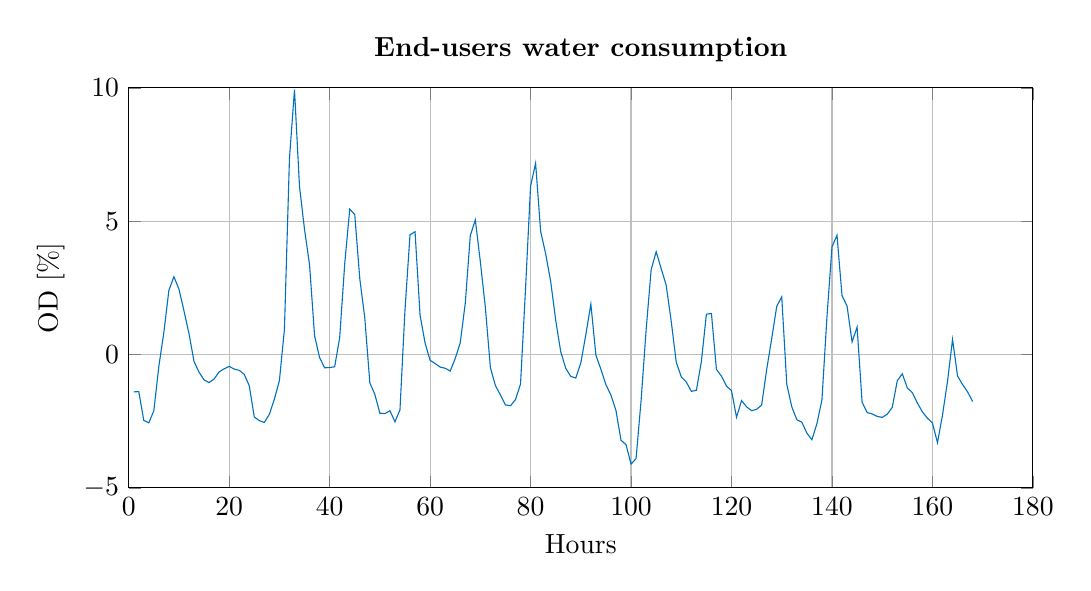
\begin{tikzpicture}

\begin{axis}[%
width=4.521in,
height=2in,
at={(1.011in,0.642in)},
scale only axis,
xmin=0,
xmax=180,
xlabel={Hours},
xmajorgrids,
ymin=-5,
ymax=10,
ylabel={OD [\%]},
ymajorgrids,
axis background/.style={fill=white},
title style={font=\bfseries},
title={End-users water consumption}
]
\addplot [color=mycolor1,solid,forget plot]
  table[row sep=crcr]{%
1	-1.40016249999999\\
2	-1.38966249999999\\
3	-2.46766249999999\\
4	-2.5611125\\
5	-2.1106625\\
6	-0.436962499999995\\
7	0.834237500000005\\
8	2.41203750000001\\
9	2.9167375\\
10	2.4533375\\
11	1.64133750000001\\
12	0.781737500000005\\
13	-0.259862499999995\\
14	-0.660262499999995\\
15	-0.952162499999994\\
16	-1.0508625\\
17	-0.915762499999995\\
18	-0.650462499999994\\
19	-0.535662499999995\\
20	-0.441862499999995\\
21	-0.546162499999995\\
22	-0.593062499999994\\
23	-0.744262499999994\\
24	-1.17091249999999\\
25	-2.3402625\\
26	-2.47851249999999\\
27	-2.54886249999999\\
28	-2.2387625\\
29	-1.67386249999999\\
30	-0.975962499999994\\
31	0.948337500000004\\
32	7.34633750000001\\
33	9.93003750000001\\
34	6.2998375\\
35	4.69053750000001\\
36	3.3675375\\
37	0.706137500000006\\
38	-0.116362499999994\\
39	-0.497162499999994\\
40	-0.486662499999996\\
41	-0.460062499999994\\
42	0.638237500000006\\
43	3.3990375\\
44	5.4556375\\
45	5.24773750000001\\
46	2.84673750000001\\
47	1.36763750000001\\
48	-1.05926249999999\\
49	-1.4974625\\
50	-2.2002625\\
51	-2.21636249999999\\
52	-2.10646249999999\\
53	-2.5236625\\
54	-2.0756625\\
55	1.6791375\\
56	4.49173750000001\\
57	4.6065375\\
58	1.47613750000001\\
59	0.429637500000005\\
60	-0.216462499999995\\
61	-0.336162499999995\\
62	-0.471262499999996\\
63	-0.513262499999995\\
64	-0.617562499999994\\
65	-0.148562499999995\\
66	0.440137500000005\\
67	1.9290375\\
68	4.46023750000001\\
69	5.0489375\\
70	3.4816375\\
71	1.76243750000001\\
72	-0.492262499999995\\
73	-1.16216249999999\\
74	-1.51636249999999\\
75	-1.8915625\\
76	-1.9174625\\
77	-1.68856249999999\\
78	-1.10546249999999\\
79	2.4883375\\
80	6.31663750000001\\
81	7.17623750000001\\
82	4.6240375\\
83	3.7801875\\
84	2.74383750000001\\
85	1.28818750000001\\
86	0.108337500000004\\
87	-0.516762499999994\\
88	-0.818812499999994\\
89	-0.881112499999995\\
90	-0.318662499999995\\
91	0.746387500000005\\
92	1.89473750000001\\
93	-0.0190624999999952\\
94	-0.553162499999995\\
95	-1.13136249999999\\
96	-1.5219625\\
97	-2.09806249999999\\
98	-3.2124625\\
99	-3.3790625\\
100	-4.1077625\\
101	-3.8998625\\
102	-1.72006249999999\\
103	0.914737500000005\\
104	3.17713750000001\\
105	3.85683750000001\\
106	3.22158750000001\\
107	2.5989375\\
108	1.24023750000001\\
109	-0.288212499999995\\
110	-0.835262499999995\\
111	-1.03021249999999\\
112	-1.3791625\\
113	-1.34276249999999\\
114	-0.264762499999995\\
115	1.51113750000001\\
116	1.54193750000001\\
117	-0.556662499999996\\
118	-0.811462499999995\\
119	-1.1866625\\
120	-1.3532625\\
121	-2.35146249999999\\
122	-1.7270625\\
123	-1.9608625\\
124	-2.10646249999999\\
125	-2.05466249999999\\
126	-1.8936625\\
127	-0.560862499999996\\
128	0.594837500000006\\
129	1.8079375\\
130	2.16213750000001\\
131	-1.1124625\\
132	-1.9608625\\
133	-2.4424625\\
134	-2.5390625\\
135	-2.94506249999999\\
136	-3.1949625\\
137	-2.5936625\\
138	-1.7032625\\
139	1.41243750000001\\
140	4.03603750000001\\
141	4.47353750000001\\
142	2.2090375\\
143	1.8233375\\
144	0.475137500000005\\
145	1.02743750000001\\
146	-1.79426249999999\\
147	-2.17436249999999\\
148	-2.2261625\\
149	-2.3199625\\
150	-2.35636249999999\\
151	-2.2366625\\
152	-1.9811625\\
153	-0.981562499999995\\
154	-0.721862499999995\\
155	-1.2524625\\
156	-1.4295625\\
157	-1.82016249999999\\
158	-2.1477625\\
159	-2.3878625\\
160	-2.56426249999999\\
161	-3.3090625\\
162	-2.27026249999999\\
163	-1.0029125\\
164	0.564037500000006\\
165	-0.805162499999995\\
166	-1.1278625\\
167	-1.39806249999999\\
168	-1.7627625\\
};
\end{axis}
\end{tikzpicture}% 
\caption{End-users water consumption, with acts as a disturbance to the system.}
\label{fig:water_consumption}
\end{figure}

In this case the model is created to last for a week based on the 24 hours data and then it repeats. 


\section{Implementation goals}
The convexity of the objective function has been developed and verified in \secref{sec:MPC} and in \secref{convexity}. 

%In this way, the main feature of this controller is the ability to reduce the cost of running the system based on the electric price and the WT level. 

Although the objective function for the minimization is convex, difficulties with infeasibility occur while solving the constrained problem. When constraints for the pressure in the WT and for the pressure in the PMAs are included, there are not any feasible solutions existing for the problem. Infeasibility means that no solution of $\bm{u_{hp}}$ exists which could satisfy all the constraints defined by the measurements carried out on the test setup. However, when constraints only on the input signals are included, the algorithm can find a global minimum of the objective function. The QP solver detects this problem automatically at the presolve phase of each optimization run, thus in these cases the MPC box does not give a solution. 

In \secref{verification_of_model}, the model is verified, however in some respects lacks the ability to give back the real world behavior of the system. As described in \secref{estim_results}, the estimation has been carried out so the dynamics of the WT reflect the same behavior as the real world system. Considering the differences between the model and the test setup, the conclusion can be made that the model is qualitatively correct but quantitatively incorrect. Although the physical limitations are calculated from the measurements on the real test setup, it should still be possible to solve the optimization with the defined constraints.

 Considering the fact that in real world completely perfect models are nearly impossible to make, blaming the accuracy of the model for infeasibility is not the right argument. It is assumed that there is a qualitative error in the two constraints concerning the WT and the output pressures. A  reason could be that there is an error in the reformulation of the original constraints for the control signal, $\bm{u_{Hp}}$. It is a reasonable assumption, since the two inequality constraints can be modified such that the optimization problem becomes feasible. However the prediction does not work as expected due to varying electricity prices not having the expected effect on the optimal control solution.

In order to present the implementation of the controller, some of the incorrect constraints are modified to show that the algorithm works and keeps the control values within the upper and lower bounds. In order to show the deficiencies of the optimization with the incorrect constraints, several results are compared and a conclusion is made concerning the expected behavior of the control. 

\section{Implementation with input constraint}
\label{input constraint}

For initial testing, the MPC is implemented such that only the constraint on the input is kept with the appropriate low and upper bounds. An implementation of such would make no sense on the test setup since the constraints on the WT are the most important boundaries concerning the control problem. In a real life scenario, leaving out the pressure constraint in the WT would mean that the optimal input empties the tank, disregarding what the price is. However, this test is suitable for verifying whether the minimization works correctly or not. It is expected to see that the input signal is constant and as low as possible during operation. This behavior, compared to the real system, is expected because the cheapest way of running the pumps is the slowest as possible. 

\begin{figure}[H]
\centering
% This file was created by matlab2tikz.
%
%The latest updates can be retrieved from
%  http://www.mathworks.com/matlabcentral/fileexchange/22022-matlab2tikz-matlab2tikz
%where you can also make suggestions and rate matlab2tikz.
%
\definecolor{mycolor1}{rgb}{0.00000,0.44700,0.74100}%
%
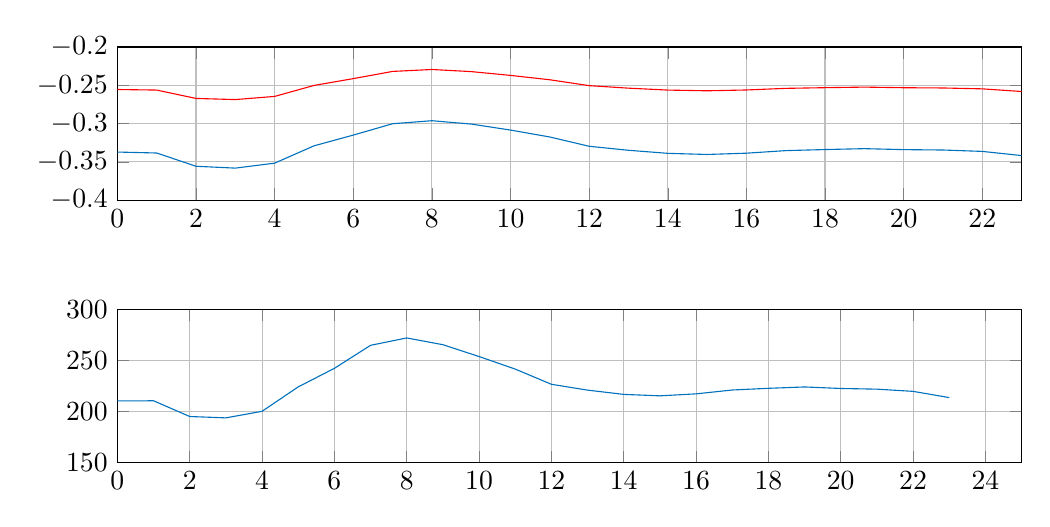
\begin{tikzpicture}

\begin{axis}[%
width=4.521in,
height=0.766in,
at={(0.758in,3.103in)},
scale only axis,
xmin=0,
xmax=23,
xmajorgrids,
ymin=-0.4,
ymax=-0.2,
ymajorgrids,
axis background/.style={fill=white}
]
\addplot [color=mycolor1,solid,forget plot]
  table[row sep=crcr]{%
0	-0.337187128298502\\
1	-0.338428175857978\\
2	-0.355759379672392\\
3	-0.358161526141837\\
4	-0.351679783260157\\
5	-0.329079947578111\\
6	-0.315052123868196\\
7	-0.30021579160496\\
8	-0.296274053706477\\
9	-0.300647937847971\\
10	-0.308494586422369\\
11	-0.317532459852742\\
12	-0.329652163199425\\
13	-0.334869915814744\\
14	-0.338864209741175\\
15	-0.340341790313779\\
16	-0.338670164645983\\
17	-0.335322051533021\\
18	-0.333915730131158\\
19	-0.332752769322142\\
20	-0.334012136632997\\
21	-0.334527251444417\\
22	-0.33633206106221\\
23	-0.341786804661069\\
};

\addplot [color=red,solid,forget plot]
  table[row sep=crcr]{%
0	-0.255539239876202\\
1	-0.25626975504531\\
2	-0.26719592758736\\
3	-0.268681742866465\\
4	-0.264551418136899\\
5	-0.250228419704096\\
6	-0.241331839560681\\
7	-0.231926715572023\\
8	-0.229416388743334\\
9	-0.232168715735042\\
10	-0.237119565456248\\
11	-0.242825434953476\\
12	-0.250482475520783\\
13	-0.253774199452117\\
14	-0.256293452004186\\
15	-0.257221941508702\\
16	-0.256159380174046\\
17	-0.254037538765411\\
18	-0.253146005750368\\
19	-0.252409936615807\\
20	-0.253208396629209\\
21	-0.253537295911981\\
22	-0.254684115730977\\
23	-0.258143242409582\\
};
\end{axis}

\begin{axis}[%
width=4.521in,
height=0.766in,
at={(0.758in,1.792in)},
scale only axis,
xmin=0,
xmax=25,
xmajorgrids,
ymin=150,
ymax=300,
ymajorgrids,
axis background/.style={fill=white}
]
\addplot [color=mycolor1,solid,forget plot]
  table[row sep=crcr]{%
0	210.15\\
1	210.3\\
2	194.9\\
3	193.565\\
4	200\\
5	223.91\\
6	242.07\\
7	264.61\\
8	271.82\\
9	265.2\\
10	253.6\\
11	241.32\\
12	226.44\\
13	220.72\\
14	216.55\\
15	215.14\\
16	217.07\\
17	220.86\\
18	222.5\\
19	223.84\\
20	222.35\\
21	221.68\\
22	219.52\\
23	213.425\\
};
\end{axis}
\end{tikzpicture}% 
\caption{Optimization only with input constraints. The first figure shows the two control inputs for the pumps. Pump one can be seen in red and pump two in blue. The second figure shows the cost of electricity for the first 24 hours.}
\label{fig:Implementation_shit}
\end{figure}

In \figref{fig:Implementation_shit} it can be seen that the full-signal input to pumps is constant at $0.05$ and $0.03$ [bar], which are the two different lower bounds for the pumps, respectively. Constraints on the pumps are set in order to avoid the lower bound hysteresis of the pumps and not to exceed the upper bound. 

As the input drops down to its minimum value, the WT level is expected to follow the same behavior and empty the water inside. In the following figure it can be seen how the WT pressure decreases until it reaches the steady-state for the input signal.

\begin{figure}[H]
\centering
% This file was created by matlab2tikz.
%
%The latest updates can be retrieved from
%  http://www.mathworks.com/matlabcentral/fileexchange/22022-matlab2tikz-matlab2tikz
%where you can also make suggestions and rate matlab2tikz.
%
\definecolor{mycolor1}{rgb}{0.00000,0.44700,0.74100}%
%
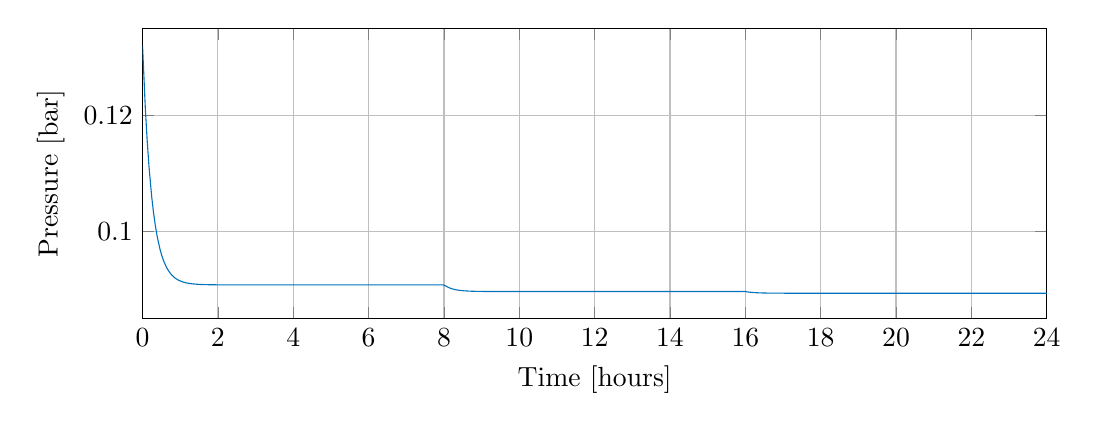
\begin{tikzpicture}

\begin{axis}[%
width=4.521in,
height=1.453in,
at={(1.011in,0.642in)},
scale only axis,
xmin=-0,
xmax=24,
xlabel={Time [hours]},
xmajorgrids,
ymin=0.085,
ymax=0.135,
ylabel={Pressure [bar]},
ymajorgrids,
axis background/.style={fill=white}
]
\addplot [color=mycolor1,solid,forget plot]
  table[row sep=crcr]{%
0	0.132\\
0.0729533333333333	0.121331836670006\\
0.121588888888889	0.115804434981837\\
0.170224444444444	0.111278980810193\\
0.243177777777778	0.105981325941061\\
0.291813333333333	0.10323649859251\\
0.340448888888889	0.10098922381935\\
0.389084444444444	0.0991493106791865\\
0.462037777777778	0.0969954440315374\\
0.510673333333333	0.0958794800388569\\
0.559308888888889	0.0949658059129309\\
0.632262222222222	0.0938962270378776\\
0.680897777777778	0.0933420555374303\\
0.729533333333333	0.0928883382449322\\
0.778168888888889	0.0925168659094808\\
0.851122222222222	0.0920820074064419\\
0.899757777777778	0.0918566979928661\\
0.948393333333333	0.0916722302296927\\
0.997028888888889	0.09152120078485\\
1.06998222222222	0.09134440043653\\
1.11861777777778	0.0912527964262102\\
1.16725333333333	0.0911777973988141\\
1.24020666666667	0.0910900009152799\\
1.28884222222222	0.0910445116950372\\
1.33747777777778	0.091007268267994\\
1.38611333333333	0.0909767759260606\\
1.45906666666667	0.0909410805245412\\
1.50770222222222	0.0909225859799307\\
1.55633777777778	0.0909074439260721\\
1.60497333333333	0.0908950466597493\\
1.67792666666667	0.0908805339863671\\
1.72656222222222	0.0908730146624806\\
1.77519777777778	0.0908668583601943\\
1.84815111111111	0.0908596515775055\\
1.89678666666667	0.0908559175905419\\
1.94542222222222	0.0908528604602961\\
1.99405777777778	0.0908503574935128\\
2.06701111111111	0.0908474274330891\\
2.11564666666667	0.0908459093066384\\
2.16428222222222	0.0908446663697094\\
2.21291777777778	0.0908436487389259\\
2.28587111111111	0.0908424574647531\\
2.33450666666667	0.0908418402403378\\
2.38314222222222	0.09084133489968\\
2.45609555555556	0.0908407433302386\\
2.50473111111111	0.0908404368255641\\
2.55336666666667	0.0908401858807375\\
2.60200222222222	0.0908399804244714\\
2.67495555555556	0.0908397399101833\\
2.72359111111111	0.0908396152946294\\
2.77222666666667	0.0908395132680335\\
2.82086222222222	0.090839429735714\\
2.89381555555556	0.0908393319498604\\
2.94245111111111	0.0908392812849357\\
2.99108666666667	0.0908392398039998\\
3.06404	0.090839191244966\\
3.11267555555556	0.0908391660855007\\
3.16131111111111	0.0908391454866708\\
3.20994666666667	0.0908391286217737\\
3.2829	0.0908391088791355\\
3.33153555555556	0.0908390986500559\\
3.38017111111111	0.0908390902751931\\
3.42880666666667	0.0908390834184347\\
3.50176	0.0908390753916736\\
3.55039555555556	0.0908390712328385\\
3.59903111111111	0.0908390678278719\\
3.67198444444444	0.090839063841899\\
3.72062	0.0908390617766819\\
3.76925555555556	0.090839060085825\\
3.81789111111111	0.0908390587014683\\
3.89084444444444	0.090839057080892\\
3.93948	0.090839056241237\\
3.98811555555556	0.0908390555537856\\
4.06106888888889	0.090839054749031\\
4.10970444444444	0.0908390543320705\\
4.15834	0.0908390539906921\\
4.20697555555556	0.0908390537111951\\
4.27992888888889	0.0908390533840061\\
4.32856444444444	0.0908390532144826\\
4.3772	0.0908390530756885\\
4.42583555555556	0.0908390529620534\\
4.49878888888889	0.0908390528290282\\
4.54742444444444	0.0908390527601051\\
4.59606	0.0908390527036756\\
4.66901333333333	0.0908390526376172\\
4.71764888888889	0.090839052603391\\
4.76628444444444	0.0908390525753689\\
4.81492	0.0908390525524264\\
4.88787333333333	0.090839052525569\\
4.93650888888889	0.0908390525116537\\
4.98514444444444	0.0908390525002607\\
5.03378	0.090839052490933\\
5.10673333333333	0.0908390524800136\\
5.15536888888889	0.090839052474356\\
5.20400444444445	0.090839052469724\\
5.27695777777778	0.0908390524643016\\
5.32559333333333	0.0908390524614921\\
5.37422888888889	0.0908390524591919\\
5.42286444444444	0.0908390524573087\\
5.49581777777778	0.0908390524551041\\
5.54445333333333	0.0908390524539619\\
5.59308888888889	0.0908390524530267\\
5.64172444444444	0.090839052452261\\
5.71467777777778	0.0908390524513647\\
5.76331333333333	0.0908390524509003\\
5.81194888888889	0.0908390524505201\\
5.88490222222222	0.090839052450075\\
5.93353777777778	0.0908390524498444\\
5.98217333333333	0.0908390524496556\\
6.03080888888889	0.090839052449501\\
6.10376222222222	0.09083905244932\\
6.15239777777778	0.0908390524492262\\
6.20103333333333	0.0908390524491495\\
6.24966888888889	0.0908390524490866\\
6.32262222222222	0.0908390524490131\\
6.37125777777778	0.0908390524489749\\
6.41989333333333	0.0908390524489437\\
6.49284666666667	0.0908390524489072\\
6.54148222222222	0.0908390524488883\\
6.59011777777778	0.0908390524488727\\
6.63875333333333	0.0908390524488601\\
6.71170666666667	0.0908390524488452\\
6.76034222222222	0.0908390524488375\\
6.80897777777778	0.0908390524488312\\
6.85761333333333	0.0908390524488261\\
6.93056666666667	0.09083905244882\\
6.97920222222222	0.0908390524488169\\
7.02783777777778	0.0908390524488143\\
7.10079111111111	0.0908390524488113\\
7.14942666666667	0.0908390524488098\\
7.19806222222222	0.0908390524488085\\
7.24669777777778	0.0908390524488075\\
7.31965111111111	0.0908390524488062\\
7.36828666666667	0.0908390524488056\\
7.41692222222222	0.0908390524488051\\
7.48987555555556	0.0908390524488045\\
7.53851111111111	0.0908390524488042\\
7.58714666666667	0.0908390524488039\\
7.63578222222222	0.0908390524488037\\
7.70873555555556	0.0908390524488035\\
7.75737111111111	0.0908390524488033\\
7.80600666666667	0.0908390524488032\\
7.85464222222222	0.0908390524488031\\
7.92759555555555	0.0908390524488031\\
7.97623111111111	0.090839052448803\\
8.02486666666667	0.0907298947843908\\
8.09782	0.0904608880972348\\
8.14645555555555	0.0903215100271097\\
8.19509111111111	0.0902073969040788\\
8.24372666666667	0.090113968972151\\
8.31668	0.0900045989686734\\
8.36531555555555	0.0899479320501836\\
8.41395111111111	0.0899015370969775\\
8.46258666666667	0.0898635521184334\\
8.53554	0.0898190855745451\\
8.58417555555556	0.0897960465150413\\
8.63281111111111	0.0897771837267325\\
8.70576444444444	0.0897551022872703\\
8.7544	0.0897436614251477\\
8.80303555555555	0.0897342944386066\\
8.85167111111111	0.0897266253979417\\
8.92462444444444	0.0897176477508196\\
8.97326	0.0897129962414339\\
9.02189555555556	0.0897091879072939\\
9.07053111111111	0.0897060699067228\\
9.14348444444444	0.0897024198662448\\
9.19212	0.0897005287028575\\
9.24075555555556	0.0896989803490878\\
9.31370888888889	0.0896971677920325\\
9.36234444444445	0.0896962286677787\\
9.41098	0.0896954597777989\\
9.45961555555556	0.0896948302638676\\
9.53256888888889	0.089694093332851\\
9.58120444444444	0.0896937115132613\\
9.62984	0.0896933989057918\\
9.67847555555555	0.0896931429644188\\
9.75142888888889	0.0896928433504995\\
9.80006444444444	0.0896926881141733\\
9.8487	0.089692561017407\\
9.92165333333333	0.089692412233489\\
9.97028888888889	0.0896923351453855\\
10.0189244444444	0.0896922720309785\\
10.06756	0.0896922203572676\\
10.1405133333333	0.0896921598662151\\
10.1891488888889	0.0896921285245179\\
10.2377844444444	0.089692102864104\\
10.28642	0.0896920818551321\\
10.3593733333333	0.0896920572612951\\
10.4080088888889	0.0896920445187065\\
10.4566444444444	0.0896920340859564\\
10.5295977777778	0.0896920218730144\\
10.5782333333333	0.0896920155452301\\
10.6268688888889	0.089692010364478\\
10.6755044444444	0.0896920061228365\\
10.7484577777778	0.0896920011574227\\
10.7970933333333	0.0896919985847365\\
10.8457288888889	0.089691996478399\\
10.9186822222222	0.0896919940126467\\
10.9673177777778	0.0896919927350881\\
11.0159533333333	0.0896919916891115\\
11.0645888888889	0.0896919908327382\\
11.1375422222222	0.0896919898302377\\
11.1861777777778	0.089691989310821\\
11.2348133333333	0.0896919888855584\\
11.2834488888889	0.0896919885373829\\
11.3564022222222	0.0896919881297964\\
11.4050377777778	0.0896919879186172\\
11.4536733333333	0.0896919877457183\\
11.5266266666667	0.0896919875433168\\
11.5752622222222	0.0896919874384483\\
11.6238977777778	0.0896919873525892\\
11.6725333333333	0.0896919872822937\\
11.7454866666667	0.0896919872000034\\
11.7941222222222	0.089691987157367\\
11.8427577777778	0.0896919871224593\\
11.8913933333333	0.0896919870938792\\
11.9643466666667	0.0896919870604225\\
12.0129822222222	0.0896919870430878\\
12.0616177777778	0.0896919870288954\\
12.1345711111111	0.0896919870122812\\
12.1832066666667	0.0896919870036731\\
12.2318422222222	0.0896919869966253\\
12.2804777777778	0.0896919869908551\\
12.3534311111111	0.0896919869841003\\
12.4020666666667	0.0896919869806005\\
12.4507022222222	0.0896919869777351\\
12.4993377777778	0.0896919869753891\\
12.5722911111111	0.0896919869726428\\
12.6209266666667	0.0896919869712199\\
12.6695622222222	0.0896919869700549\\
12.7425155555556	0.0896919869686911\\
12.7911511111111	0.0896919869679845\\
12.8397866666667	0.089691986967406\\
12.8884222222222	0.0896919869669324\\
12.9613755555556	0.0896919869663779\\
13.0100111111111	0.0896919869660906\\
13.0586466666667	0.0896919869658554\\
13.1072822222222	0.0896919869656628\\
13.1802355555556	0.0896919869654374\\
13.2288711111111	0.0896919869653206\\
13.2775066666667	0.089691986965225\\
13.35046	0.089691986965113\\
13.3990955555556	0.089691986965055\\
13.4477311111111	0.0896919869650075\\
13.4963666666667	0.0896919869649687\\
13.56932	0.0896919869649231\\
13.6179555555556	0.0896919869648996\\
13.6665911111111	0.0896919869648803\\
13.7152266666667	0.0896919869648644\\
13.78818	0.0896919869648459\\
13.8368155555556	0.0896919869648364\\
13.8854511111111	0.0896919869648285\\
13.9584044444444	0.0896919869648193\\
14.00704	0.0896919869648146\\
14.0556755555556	0.0896919869648107\\
14.1043111111111	0.0896919869648075\\
14.1772644444444	0.0896919869648037\\
14.2259	0.0896919869648018\\
14.2745355555556	0.0896919869648002\\
14.3474888888889	0.0896919869647984\\
14.3961244444444	0.0896919869647974\\
14.44476	0.0896919869647966\\
14.4933955555556	0.089691986964796\\
14.5663488888889	0.0896919869647952\\
14.6149844444444	0.0896919869647948\\
14.66362	0.0896919869647945\\
14.7122555555556	0.0896919869647942\\
14.7852088888889	0.0896919869647939\\
14.8338444444444	0.0896919869647938\\
14.88248	0.0896919869647936\\
14.9554333333333	0.0896919869647935\\
15.0040688888889	0.0896919869647934\\
15.0527044444444	0.0896919869647934\\
15.10134	0.0896919869647933\\
15.1742933333333	0.0896919869647932\\
15.2229288888889	0.0896919869647932\\
15.2715644444444	0.0896919869647932\\
15.2958822222222	0.0896919869647932\\
15.3202	0.0896919869647932\\
15.3688355555556	0.0896919869647931\\
15.3931533333333	0.0896919869647931\\
15.4417888888889	0.0896919869647931\\
15.4661066666667	0.0896919869647931\\
15.4904244444444	0.0896919869647931\\
15.5633777777778	0.0896919869647931\\
15.6120133333333	0.0896919869647931\\
15.6606488888889	0.0896919869647931\\
15.7092844444444	0.0896919869647931\\
15.7822377777778	0.0896919869647931\\
15.8308733333333	0.0896919869647931\\
15.8795088888889	0.0896919869647931\\
15.9281444444444	0.0896919869647931\\
16.0010977777778	0.0896919869647931\\
16.0497333333333	0.0896397386189188\\
16.0983688888889	0.0895969612873375\\
16.1713222222222	0.0895468846474368\\
16.2199577777778	0.0895209388782015\\
16.2685933333333	0.0894996962770216\\
16.3172288888889	0.0894823043045273\\
16.3901822222222	0.0894619446534792\\
16.4388177777778	0.0894513958864523\\
16.4874533333333	0.0894427592856693\\
16.5360888888889	0.0894356882343423\\
16.6090422222222	0.0894274106144457\\
16.6576777777778	0.0894231218040127\\
16.7063133333333	0.0894196104226874\\
16.7792666666667	0.0894154998769455\\
16.8279022222222	0.0894133701160138\\
16.8765377777778	0.0894116264150786\\
16.9251733333333	0.0894101987933647\\
16.9981266666667	0.0894085275694749\\
17.0467622222222	0.0894076616729317\\
17.0953977777778	0.0894069527367363\\
17.1440333333333	0.0894063723088166\\
17.2169866666667	0.0894056928396013\\
17.2656222222222	0.0894053407921896\\
17.3142577777778	0.08940505256012\\
17.3872111111111	0.0894047151455824\\
17.4358466666667	0.0894045403239541\\
17.4844822222222	0.0894043971920972\\
17.5331177777778	0.0894042800056332\\
17.6060711111111	0.0894041428230615\\
17.6547066666667	0.0894040717458616\\
17.7033422222222	0.0894040135527666\\
17.7762955555556	0.0894039454298952\\
17.8249311111111	0.0894039101339907\\
17.8735666666667	0.0894038812361454\\
17.9222022222222	0.0894038575765886\\
17.9951555555556	0.0894038298798843\\
18.0437911111111	0.0894038155296343\\
18.0924266666667	0.0894038037806422\\
18.1410622222222	0.0894037941613802\\
18.2140155555556	0.0894037829007358\\
18.2626511111111	0.0894037770663571\\
18.3112866666667	0.0894037722895713\\
18.38424	0.089403766697699\\
18.4328755555556	0.0894037638004313\\
18.4815111111111	0.0894037614283489\\
18.5301466666667	0.089403759486252\\
18.6031	0.0894037572127653\\
18.6517355555556	0.0894037560348237\\
18.7003711111111	0.0894037550704066\\
18.7490066666667	0.0894037542808086\\
18.82196	0.0894037533564775\\
18.8705955555556	0.089403752877562\\
18.9192311111111	0.089403752485459\\
18.9921844444444	0.0894037520264497\\
19.04082	0.0894037517886272\\
19.0894555555556	0.0894037515939146\\
19.1380911111111	0.0894037514344974\\
19.2110444444444	0.089403751247878\\
19.25968	0.0894037511511866\\
19.3083155555556	0.0894037510720223\\
19.3569511111111	0.0894037510072081\\
19.4299044444444	0.0894037509313343\\
19.47854	0.0894037508920224\\
19.5271755555556	0.0894037508598366\\
19.6001288888889	0.0894037508221588\\
19.6487644444444	0.0894037508026371\\
19.6974	0.0894037507866541\\
19.7460355555556	0.0894037507735683\\
19.8189888888889	0.0894037507582497\\
19.8676244444444	0.0894037507503127\\
19.91626	0.0894037507438145\\
19.9648955555556	0.0894037507384942\\
20.0378488888889	0.0894037507322661\\
20.0864844444444	0.0894037507290392\\
20.13512	0.0894037507263972\\
20.2080733333333	0.0894037507233044\\
20.2567088888889	0.089403750721702\\
20.3053444444444	0.08940375072039\\
20.35398	0.0894037507193159\\
20.4269333333333	0.0894037507180585\\
20.4755688888889	0.089403750717407\\
20.5242044444444	0.0894037507168736\\
20.57284	0.0894037507164368\\
20.6457933333333	0.0894037507159256\\
20.6944288888889	0.0894037507156607\\
20.7430644444444	0.0894037507154438\\
20.8160177777778	0.08940375071519\\
20.8646533333333	0.0894037507150584\\
20.9132888888889	0.0894037507149508\\
20.9619244444444	0.0894037507148626\\
21.0348777777778	0.0894037507147594\\
21.0835133333333	0.0894037507147059\\
21.1321488888889	0.0894037507146621\\
21.2051022222222	0.0894037507146109\\
21.2537377777778	0.0894037507145843\\
21.3023733333333	0.0894037507145626\\
21.3510088888889	0.0894037507145448\\
21.4239622222222	0.0894037507145239\\
21.4725977777778	0.0894037507145131\\
21.5212333333333	0.0894037507145043\\
21.5698688888889	0.089403750714497\\
21.6428222222222	0.0894037507144886\\
21.6914577777778	0.0894037507144842\\
21.7400933333333	0.0894037507144806\\
21.8130466666667	0.0894037507144764\\
21.8616822222222	0.0894037507144742\\
21.9103177777778	0.0894037507144724\\
21.9589533333333	0.0894037507144709\\
22.0319066666667	0.0894037507144692\\
22.0805422222222	0.0894037507144683\\
22.1291777777778	0.0894037507144676\\
22.1778133333333	0.089403750714467\\
22.2507666666667	0.0894037507144663\\
22.2994022222222	0.089403750714466\\
22.3480377777778	0.0894037507144657\\
22.4209911111111	0.0894037507144653\\
22.4696266666667	0.0894037507144652\\
22.5182622222222	0.089403750714465\\
22.5668977777778	0.0894037507144649\\
22.6398511111111	0.0894037507144647\\
22.6884866666667	0.0894037507144647\\
22.7371222222222	0.0894037507144646\\
22.7857577777778	0.0894037507144646\\
22.8587111111111	0.0894037507144645\\
22.9073466666667	0.0894037507144645\\
22.9559822222222	0.0894037507144645\\
23.0289355555556	0.0894037507144644\\
23.0532533333333	0.0894037507144644\\
23.0775711111111	0.0894037507144644\\
23.1262066666667	0.0894037507144644\\
23.1748422222222	0.0894037507144644\\
23.2477955555556	0.0894037507144644\\
23.2964311111111	0.0894037507144644\\
23.3450666666667	0.0894037507144644\\
23.3937022222222	0.0894037507144644\\
23.4666555555556	0.0894037507144644\\
23.5152911111111	0.0894037507144644\\
23.5639266666667	0.0894037507144644\\
23.63688	0.0894037507144644\\
23.6855155555556	0.0894037507144644\\
23.7341511111111	0.0894037507144644\\
23.7827866666667	0.0894037507144644\\
23.85574	0.0894037507144644\\
23.9043755555556	0.0894037507144644\\
24.0016466666667	0.0894037507144644\\
};
\end{axis}
\end{tikzpicture}% 
\caption{WT pressure for simulation with input constraint.}
\label{fig:WT_input}
\end{figure}

The initial pressure in the WT from $0.132$ [bar] drops and shows the dynamics of how the tank is being emptied. Since the optimal solution for the control signal is bounded by the lower constraint, the WT is not emptied completely. This result is reasonable and expected, as the lower constraints for the pumps are small values and the initial condition set for the WT is significantly high. The pressure in the WT is dominant in the system, compared to the pressure provided by the pumps, thus the water level decreases.

The PMA pressures also experience a pressure drop due to the decrease in the control input in the pumps, as seen in \figref{fig:Output_input}.

\begin{figure}[H]
\centering
% This file was created by matlab2tikz.
%
%The latest updates can be retrieved from
%  http://www.mathworks.com/matlabcentral/fileexchange/22022-matlab2tikz-matlab2tikz
%where you can also make suggestions and rate matlab2tikz.
%
\definecolor{mycolor1}{rgb}{0.00000,0.44700,0.74100}%
\definecolor{mycolor2}{rgb}{0.85000,0.32500,0.09800}%
%
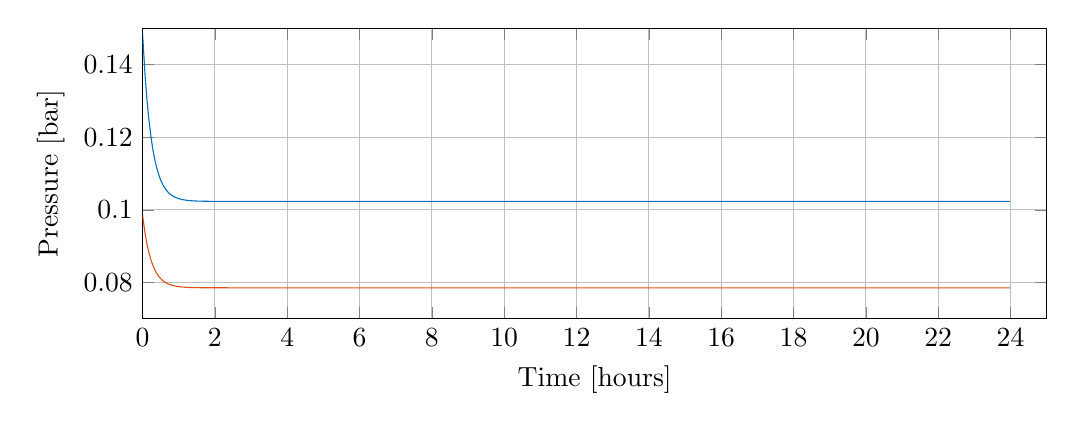
\begin{tikzpicture}

\begin{axis}[%
scaled y ticks = false,
 y tick label style={/pgf/number format/fixed,
/pgf/number format/1000 sep = \thinspace}, % Optional if you want to replace comma as the 1000 separator 
width=4.521in,
height=1.453in,
at={(1.011in,0.642in)},
scale only axis,
xmin=0,
xmax=25,
xlabel={Time [hours]},
xmajorgrids,
ymin=0.07,
ymax=0.15,
ylabel={Pressure [bar]},
ymajorgrids,
axis background/.style={fill=white}
]
\addplot [color=mycolor1,solid,forget plot]
  table[row sep=crcr]{%
0	0.148573348643486\\
0.0729533333333333	0.136586914061809\\
0.121588888888889	0.130376488078208\\
0.170224444444444	0.12529182086145\\
0.243177777777778	0.11933953165109\\
0.291813333333333	0.116255524362496\\
0.340448888888889	0.113730552515571\\
0.389084444444444	0.111663280219728\\
0.462037777777778	0.109243258995666\\
0.510673333333333	0.107989394671928\\
0.559308888888889	0.106962817293505\\
0.607944444444444	0.106122326744457\\
0.680897777777778	0.10513841912309\\
0.729533333333333	0.10462863571624\\
0.778168888888889	0.1042112603388\\
0.851122222222222	0.103722666105143\\
0.899757777777778	0.103469515072831\\
0.948393333333333	0.103262252518044\\
0.997028888888889	0.103092560274544\\
1.06998222222222	0.102893912601641\\
1.11861777777778	0.102790989029083\\
1.16725333333333	0.102706722327101\\
1.21588888888889	0.102637730580249\\
1.28884222222222	0.102556966429343\\
1.33747777777778	0.102515120812952\\
1.38611333333333	0.102480860519895\\
1.45906666666667	0.102440754213105\\
1.50770222222222	0.102419974285536\\
1.55633777777778	0.102402961118191\\
1.60497333333333	0.102389031913571\\
1.67792666666667	0.102372725899659\\
1.72656222222222	0.102364277408008\\
1.77519777777778	0.102357360367427\\
1.82383333333333	0.102351697173051\\
1.89678666666667	0.102345067639737\\
1.94542222222222	0.102341632752268\\
1.99405777777778	0.102338820484942\\
2.06701111111111	0.102335528353161\\
2.11564666666667	0.102333822629891\\
2.16428222222222	0.102332426101663\\
2.21291777777778	0.102331282720948\\
2.28587111111111	0.102329944239509\\
2.33450666666667	0.102329250743887\\
2.38314222222222	0.102328682957641\\
2.43177777777778	0.102328218093536\\
2.50473111111111	0.102327673910527\\
2.55336666666667	0.102327391961901\\
2.60200222222222	0.102327161114551\\
2.67495555555556	0.10232689087796\\
2.72359111111111	0.102326750862652\\
2.77222666666667	0.102326636227802\\
2.82086222222222	0.102326542372716\\
2.89381555555556	0.102326432502672\\
2.94245111111111	0.102326375576672\\
2.99108666666667	0.1023263289696\\
3.03972222222222	0.102326290810954\\
3.11267555555556	0.102326246155481\\
3.16131111111111	0.102326223003784\\
3.20994666666667	0.102326204053424\\
3.2829	0.102326181869541\\
3.33153555555556	0.1023261703756\\
3.38017111111111	0.102326160965156\\
3.42880666666667	0.102326153260536\\
3.50176	0.102326144241238\\
3.55039555555556	0.102326139568149\\
3.59903111111111	0.102326135742146\\
3.64766666666667	0.102326132609695\\
3.72062	0.102326128951642\\
3.76925555555556	0.102326127049114\\
3.81789111111111	0.102326125492425\\
3.89084444444444	0.102326123670113\\
3.93948	0.102326122725934\\
3.98811555555556	0.102326121952906\\
4.03675111111111	0.102326121320004\\
4.10970444444444	0.102326120579107\\
4.15834	0.102326120195232\\
4.20697555555556	0.102326119880942\\
4.25561111111111	0.102326119626788\\
4.32856444444444	0.102326119329467\\
4.3772	0.102326119172065\\
4.42583555555556	0.102326119043243\\
4.49878888888889	0.102326118892441\\
4.54742444444444	0.102326118814307\\
4.59606	0.102326118750336\\
4.64469555555555	0.102326118697961\\
4.71764888888889	0.102326118636649\\
4.76628444444444	0.102326118604883\\
4.81492	0.102326118578888\\
4.83923777777778	0.102326118570859\\
4.86355555555556	0.102326118571952\\
4.93650888888889	0.102326118538998\\
4.98514444444444	0.10232611852493\\
5.03378	0.102326118513415\\
5.10673333333333	0.102326118499934\\
5.15536888888889	0.102326118492949\\
5.20400444444445	0.102326118487231\\
5.25264	0.102326118482549\\
5.32559333333333	0.102326118477068\\
5.37422888888889	0.102326118474228\\
5.39854666666667	0.102326118473022\\
5.42286444444444	0.102326118475068\\
5.44718222222222	0.102326118485276\\
5.4715	0.102326118478936\\
5.54445333333333	0.102326118473511\\
5.59308888888889	0.102326118471316\\
5.64172444444444	0.102326118469519\\
5.71467777777778	0.102326118467415\\
5.76331333333333	0.102326118466325\\
5.81194888888889	0.102326118465433\\
5.86058444444444	0.102326118464702\\
5.93353777777778	0.102326118463847\\
5.98217333333333	0.102326118463418\\
6.03080888888889	0.102326118477413\\
6.07944444444444	0.102326118469814\\
6.15239777777778	0.102326118467589\\
6.20103333333333	0.102326118466468\\
6.24966888888889	0.10232611846555\\
6.29830444444444	0.102326118464798\\
6.37125777777778	0.102326118463918\\
6.41989333333333	0.102326118463462\\
6.46852888888889	0.102326118463088\\
6.54148222222222	0.102326118462651\\
6.5658	0.102326118462547\\
6.59011777777778	0.102326118465589\\
6.61443555555556	0.1023261184767\\
6.63875333333333	0.102326118471176\\
6.68738888888889	0.102326118468433\\
6.76034222222222	0.102326118466609\\
6.80897777777778	0.102326118465665\\
6.85761333333333	0.102326118464893\\
6.90624888888889	0.10232611846426\\
6.97920222222222	0.102326118463519\\
7.02783777777778	0.102326118463135\\
7.07647333333333	0.102326118462821\\
7.14942666666667	0.102326118462468\\
7.19806222222222	0.102326118476635\\
7.24669777777778	0.102326118469177\\
7.29533333333333	0.102326118467719\\
7.36828666666667	0.102326118466082\\
7.41692222222222	0.102326118465233\\
7.46555777777778	0.102326118464539\\
7.51419333333333	0.10232611846397\\
7.58714666666667	0.102326118463305\\
7.63578222222222	0.10232611846296\\
7.68441777777778	0.102326118462677\\
7.73305333333333	0.102326118462461\\
7.75737111111111	0.102326118465511\\
7.78168888888889	0.102326118476629\\
7.80600666666667	0.102326118471112\\
7.85464222222222	0.102326118468381\\
7.90327777777778	0.102326118467114\\
7.97623111111111	0.102326118465634\\
8.02486666666667	0.102326118464867\\
8.07350222222222	0.102326118464239\\
8.12213777777778	0.102326118463724\\
8.19509111111111	0.102326118463123\\
8.24372666666667	0.102326118462811\\
8.29236222222222	0.102326118462555\\
8.31668	0.10232611846246\\
8.36531555555555	0.102326118476629\\
8.41395111111111	0.102326118469172\\
8.46258666666667	0.102326118467714\\
8.51122222222222	0.10232611846657\\
8.58417555555556	0.102326118465231\\
8.63281111111111	0.102326118464537\\
8.68144666666667	0.102326118463968\\
8.73008222222222	0.102326118463503\\
8.80303555555555	0.102326118462959\\
8.85167111111111	0.102326118462677\\
8.90030666666667	0.10232611846246\\
8.94894222222222	0.102326118476629\\
8.97326	0.102326118471111\\
9.02189555555556	0.10232611846838\\
9.07053111111111	0.102326118467114\\
9.11916666666667	0.102326118466078\\
9.19212	0.102326118464866\\
9.24075555555556	0.102326118464238\\
9.28939111111111	0.102326118463724\\
9.33802666666667	0.102326118463303\\
9.41098	0.102326118462811\\
9.45961555555556	0.102326118462555\\
9.48393333333333	0.10232611846246\\
9.50825111111111	0.102326118465511\\
9.53256888888889	0.102326118476629\\
9.58120444444444	0.102326118469172\\
9.62984	0.102326118467714\\
9.67847555555555	0.10232611846657\\
9.72711111111111	0.102326118465633\\
9.80006444444444	0.102326118464537\\
9.8487	0.102326118463968\\
9.89733555555555	0.102326118463503\\
9.94597111111111	0.102326118463122\\
10.0189244444444	0.102326118462677\\
10.06756	0.10232611846246\\
10.1161955555556	0.102326118476629\\
10.1891488888889	0.10232611846838\\
10.2377844444444	0.102326118467114\\
10.28642	0.102326118466078\\
10.3350555555556	0.102326118465231\\
10.4080088888889	0.102326118464238\\
10.4566444444444	0.102326118463724\\
10.50528	0.102326118463303\\
10.5539155555556	0.102326118462959\\
10.6268688888889	0.102326118462555\\
10.6511866666667	0.10232611846246\\
10.6755044444444	0.102326118465511\\
10.6998222222222	0.102326118476629\\
10.72414	0.102326118471111\\
10.7970933333333	0.102326118467714\\
10.8457288888889	0.10232611846657\\
10.8943644444444	0.102326118465633\\
10.943	0.102326118464866\\
11.0159533333333	0.102326118463968\\
11.0645888888889	0.102326118463503\\
11.1132244444444	0.102326118463122\\
11.16186	0.102326118462811\\
11.2348133333333	0.10232611846246\\
11.2834488888889	0.102326118476629\\
11.3320844444444	0.102326118469172\\
11.4050377777778	0.102326118467114\\
11.4536733333333	0.102326118466078\\
11.5023088888889	0.102326118465231\\
11.5509444444444	0.102326118464537\\
11.6238977777778	0.102326118463724\\
11.6725333333333	0.102326118463303\\
11.7211688888889	0.102326118462959\\
11.7698044444444	0.102326118462677\\
11.81844	0.10232611846246\\
11.8427577777778	0.102326118465511\\
11.8670755555556	0.102326118476629\\
11.8913933333333	0.102326118471111\\
11.9400288888889	0.10232611846838\\
12.0129822222222	0.10232611846657\\
12.0616177777778	0.102326118465633\\
12.1102533333333	0.102326118464866\\
12.1588888888889	0.102326118464238\\
12.2318422222222	0.102326118463503\\
12.2804777777778	0.102326118463122\\
12.3291133333333	0.102326118462811\\
12.3777488888889	0.102326118462555\\
12.4020666666667	0.10232611846246\\
12.4507022222222	0.102326118476629\\
12.4993377777778	0.102326118469172\\
12.5479733333333	0.102326118467714\\
12.5966088888889	0.10232611846657\\
12.6695622222222	0.102326118465231\\
12.7181977777778	0.102326118464537\\
12.7668333333333	0.102326118463968\\
12.8397866666667	0.102326118463303\\
12.8884222222222	0.102326118462959\\
12.9370577777778	0.102326118462677\\
12.9856933333333	0.10232611846246\\
13.0343288888889	0.102326118476629\\
13.0586466666667	0.102326118471111\\
13.1072822222222	0.10232611846838\\
13.1559177777778	0.102326118467114\\
13.2045533333333	0.102326118466078\\
13.2775066666667	0.102326118464866\\
13.3261422222222	0.102326118464238\\
13.3747777777778	0.102326118463724\\
13.4477311111111	0.102326118463122\\
13.4963666666667	0.102326118462811\\
13.5450022222222	0.102326118462555\\
13.56932	0.10232611846246\\
13.5936377777778	0.102326118465511\\
13.6179555555556	0.102326118476629\\
13.6665911111111	0.102326118469172\\
13.7152266666667	0.102326118467714\\
13.7638622222222	0.10232611846657\\
13.8124977777778	0.102326118465633\\
13.8854511111111	0.102326118464537\\
13.9340866666667	0.102326118463968\\
13.9827222222222	0.102326118463503\\
14.0556755555556	0.102326118462959\\
14.1043111111111	0.102326118462677\\
14.1529466666667	0.10232611846246\\
14.2015822222222	0.102326118476629\\
14.2745355555556	0.10232611846838\\
14.3231711111111	0.102326118467114\\
14.3718066666667	0.102326118466078\\
14.4204422222222	0.102326118465231\\
14.4933955555556	0.102326118464238\\
14.5420311111111	0.102326118463724\\
14.5906666666667	0.102326118463303\\
14.66362	0.102326118462811\\
14.7122555555556	0.102326118462555\\
14.7365733333333	0.10232611846246\\
14.7608911111111	0.102326118465511\\
14.7852088888889	0.102326118476629\\
14.8095266666667	0.102326118471111\\
14.88248	0.102326118467714\\
14.9311155555556	0.10232611846657\\
14.9797511111111	0.102326118465633\\
15.0283866666667	0.102326118464866\\
15.10134	0.102326118463968\\
15.1499755555556	0.102326118463503\\
15.1986111111111	0.102326118463122\\
15.2715644444444	0.102326118462677\\
15.3202	0.10232611846246\\
15.3688355555556	0.102326118476629\\
15.4174711111111	0.102326118469172\\
15.4904244444444	0.102326118467114\\
15.53906	0.102326118466078\\
15.5876955555556	0.102326118465231\\
15.6363311111111	0.102326118464537\\
15.7092844444444	0.102326118463724\\
15.75792	0.102326118463303\\
15.8065555555556	0.102326118462959\\
15.8795088888889	0.102326118462555\\
15.9038266666667	0.10232611846246\\
15.9281444444444	0.102326118465511\\
15.9524622222222	0.102326118476629\\
15.97678	0.102326118471111\\
16.0254155555556	0.10232611846838\\
16.0983688888889	0.10232611846657\\
16.1470044444444	0.102326118465633\\
16.19564	0.102326118464866\\
16.2442755555556	0.102326118464238\\
16.3172288888889	0.102326118463503\\
16.3658644444444	0.102326118463122\\
16.4145	0.102326118462811\\
16.4874533333333	0.10232611846246\\
16.5360888888889	0.102326118476629\\
16.5847244444444	0.102326118469172\\
16.63336	0.102326118467714\\
16.7063133333333	0.102326118466078\\
16.7549488888889	0.102326118465231\\
16.8035844444444	0.102326118464537\\
16.85222	0.102326118463968\\
16.9251733333333	0.102326118463303\\
16.9738088888889	0.102326118462959\\
17.0224444444444	0.102326118462677\\
17.07108	0.10232611846246\\
17.0953977777778	0.102326118465511\\
17.1197155555556	0.102326118476629\\
17.1440333333333	0.102326118471111\\
17.1926688888889	0.10232611846838\\
17.2413044444444	0.102326118467114\\
17.3142577777778	0.102326118465633\\
17.3628933333333	0.102326118464866\\
17.4115288888889	0.102326118464238\\
17.4601644444444	0.102326118463724\\
17.5331177777778	0.102326118463122\\
17.5817533333333	0.102326118462811\\
17.6303888888889	0.102326118462555\\
17.6547066666667	0.10232611846246\\
17.7033422222222	0.102326118476629\\
17.7519777777778	0.102326118469172\\
17.8006133333333	0.102326118467714\\
17.8492488888889	0.10232611846657\\
17.9222022222222	0.102326118465231\\
17.9708377777778	0.102326118464537\\
18.0194733333333	0.102326118463968\\
18.0681088888889	0.102326118463503\\
18.1410622222222	0.102326118462959\\
18.1896977777778	0.102326118462677\\
18.2383333333333	0.10232611846246\\
18.2869688888889	0.102326118476629\\
18.3599222222222	0.10232611846838\\
18.4085577777778	0.102326118467114\\
18.4571933333333	0.102326118466078\\
18.5301466666667	0.102326118464866\\
18.5787822222222	0.102326118464238\\
18.6274177777778	0.102326118463724\\
18.6760533333333	0.102326118463303\\
18.7490066666667	0.102326118462811\\
18.7976422222222	0.102326118462555\\
18.82196	0.10232611846246\\
18.8462777777778	0.102326118465511\\
18.8705955555556	0.102326118476629\\
18.8949133333333	0.102326118471111\\
18.9678666666667	0.102326118467714\\
19.0165022222222	0.10232611846657\\
19.0651377777778	0.102326118465633\\
19.1380911111111	0.102326118464537\\
19.1867266666667	0.102326118463968\\
19.2353622222222	0.102326118463503\\
19.2839977777778	0.102326118463122\\
19.3569511111111	0.102326118462677\\
19.4055866666667	0.10232611846246\\
19.4542222222222	0.102326118476629\\
19.5028577777778	0.102326118469172\\
19.5758111111111	0.102326118467114\\
19.6244466666667	0.102326118466078\\
19.6730822222222	0.102326118465231\\
19.7460355555556	0.102326118464238\\
19.7946711111111	0.102326118463724\\
19.8433066666667	0.102326118463303\\
19.8919422222222	0.102326118462959\\
19.9648955555556	0.102326118462555\\
19.9892133333333	0.10232611846246\\
20.0135311111111	0.102326118465511\\
20.0378488888889	0.102326118476629\\
20.0621666666667	0.102326118471111\\
20.1108022222222	0.10232611846838\\
20.1837555555556	0.10232611846657\\
20.2323911111111	0.102326118465633\\
20.2810266666667	0.102326118464866\\
20.35398	0.102326118463968\\
20.4026155555556	0.102326118463503\\
20.4512511111111	0.102326118463122\\
20.4998866666667	0.102326118462811\\
20.57284	0.10232611846246\\
20.6214755555556	0.102326118476629\\
20.6701111111111	0.102326118469172\\
20.7187466666667	0.102326118467714\\
20.7917	0.102326118466078\\
20.8403355555556	0.102326118465231\\
20.8889711111111	0.102326118464537\\
20.9619244444444	0.102326118463724\\
21.01056	0.102326118463303\\
21.0591955555556	0.102326118462959\\
21.1078311111111	0.102326118462677\\
21.1564666666667	0.10232611846246\\
21.1807844444444	0.102326118465511\\
21.2051022222222	0.102326118476629\\
21.22942	0.102326118471111\\
21.2780555555556	0.10232611846838\\
21.3266911111111	0.102326118467114\\
21.3996444444444	0.102326118465633\\
21.44828	0.102326118464866\\
21.4969155555556	0.102326118464238\\
21.5698688888889	0.102326118463503\\
21.6185044444444	0.102326118463122\\
21.66714	0.102326118462811\\
21.7157755555556	0.102326118462555\\
21.7400933333333	0.10232611846246\\
21.7887288888889	0.102326118476629\\
21.8373644444444	0.102326118469172\\
21.886	0.102326118467714\\
21.9346355555556	0.10232611846657\\
22.0075888888889	0.102326118465231\\
22.0562244444444	0.102326118464537\\
22.10486	0.102326118463968\\
22.1778133333333	0.102326118463303\\
22.2264488888889	0.102326118462959\\
22.2750844444444	0.102326118462677\\
22.32372	0.10232611846246\\
22.3723555555556	0.102326118476629\\
22.3966733333333	0.102326118471111\\
22.4453088888889	0.10232611846838\\
22.4939444444444	0.102326118467114\\
22.54258	0.102326118466078\\
22.6155333333333	0.102326118464866\\
22.6641688888889	0.102326118464238\\
22.7128044444444	0.102326118463724\\
22.7857577777778	0.102326118463122\\
22.8343933333333	0.102326118462811\\
22.8830288888889	0.102326118462555\\
22.9073466666667	0.10232611846246\\
22.9316644444444	0.102326118465511\\
22.9559822222222	0.102326118476629\\
23.0046177777778	0.102326118469172\\
23.0532533333333	0.102326118467714\\
23.1018888888889	0.10232611846657\\
23.1505244444444	0.102326118465633\\
23.2234777777778	0.102326118464537\\
23.2721133333333	0.102326118463968\\
23.3207488888889	0.102326118463503\\
23.3937022222222	0.102326118462959\\
23.4423377777778	0.102326118462677\\
23.4909733333333	0.10232611846246\\
23.5396088888889	0.102326118476629\\
23.6125622222222	0.10232611846838\\
23.6611977777778	0.102326118467114\\
23.7098333333333	0.102326118466078\\
23.7584688888889	0.102326118465231\\
23.8314222222222	0.102326118464238\\
23.8800577777778	0.102326118463724\\
23.9286933333333	0.102326118463303\\
23.9773288888889	0.102326118462959\\
};
\addplot [color=mycolor2,solid,forget plot]
  table[row sep=crcr]{%
0	0.0984938461450145\\
0.0729533333333333	0.0933215078517142\\
0.121588888888889	0.090641609679009\\
0.170224444444444	0.088447494424006\\
0.243177777777778	0.0858789864000841\\
0.291813333333333	0.0845481879139811\\
0.340448888888889	0.0834586221649368\\
0.389084444444444	0.0825665610949323\\
0.462037777777778	0.0815222832187616\\
0.510673333333333	0.080981220702458\\
0.559308888888889	0.0805382361394278\\
0.607944444444444	0.0801755510204812\\
0.680897777777778	0.0797509791402956\\
0.729533333333333	0.0795309994441952\\
0.778168888888889	0.0793508952861208\\
0.851122222222222	0.0791400590623773\\
0.899757777777778	0.0790308203417656\\
0.948393333333333	0.0789413832333755\\
0.997028888888889	0.0788681583153946\\
1.06998222222222	0.0787824386663671\\
1.11861777777778	0.0787380254981311\\
1.16725333333333	0.0787016630680404\\
1.21588888888889	0.078671892025473\\
1.28884222222222	0.0786370410022091\\
1.33747777777778	0.0786189839480097\\
1.38611333333333	0.0786042000837558\\
1.45906666666667	0.0785868935716198\\
1.50770222222222	0.0785779267004152\\
1.55633777777778	0.0785705852465118\\
1.60497333333333	0.0785645745718644\\
1.67792666666667	0.0785575382659811\\
1.72656222222222	0.0785538926066661\\
1.77519777777778	0.0785509077929894\\
1.82383333333333	0.0785484640340106\\
1.89678666666667	0.0785456032843136\\
1.94542222222222	0.0785441210703075\\
1.99405777777778	0.0785429075370318\\
2.06701111111111	0.0785414869295423\\
2.11564666666667	0.0785407508826617\\
2.16428222222222	0.0785401482583883\\
2.21291777777778	0.0785396548713167\\
2.28587111111111	0.0785390772951613\\
2.33450666666667	0.078538778040705\\
2.38314222222222	0.0785385330318557\\
2.43177777777778	0.0785383324355571\\
2.50473111111111	0.078538097610645\\
2.55336666666667	0.0785379759456332\\
2.60200222222222	0.078537876332213\\
2.67495555555556	0.078537759720802\\
2.72359111111111	0.0785376993019563\\
2.77222666666667	0.0785376498351847\\
2.82086222222222	0.0785376093352136\\
2.89381555555556	0.0785375619245317\\
2.94245111111111	0.0785375373600517\\
2.99108666666667	0.0785375172483547\\
3.03972222222222	0.0785375007822883\\
3.11267555555556	0.0785374815076233\\
3.16131111111111	0.0785374715223648\\
3.20994666666667	0.0785374633450263\\
3.2829	0.0785374537723256\\
3.33153555555556	0.0785374488125063\\
3.38017111111111	0.0785374447517494\\
3.42880666666667	0.0785374414270825\\
3.50176	0.0785374375351111\\
3.55039555555556	0.0785374355185983\\
3.59903111111111	0.078537433867617\\
3.64766666666667	0.0785374325159083\\
3.72062	0.0785374309364997\\
3.76925555555556	0.0785374301164329\\
3.81789111111111	0.0785374294446981\\
3.89084444444444	0.0785374286583413\\
3.93948	0.0785374282509131\\
3.98811555555556	0.0785374279173391\\
4.03675111111111	0.0785374276442317\\
4.10970444444444	0.0785374273245228\\
4.15834	0.0785374271588748\\
4.20697555555556	0.0785374270232536\\
4.25561111111111	0.0785374269123445\\
4.32856444444444	0.0785374267852383\\
4.3772	0.0785374267173616\\
4.42583555555556	0.0785374266617732\\
4.49878888888889	0.0785374265966995\\
4.54742444444444	0.0785374265629834\\
4.59606	0.078537426535379\\
4.64469555555555	0.0785374265127784\\
4.71764888888889	0.0785374264863214\\
4.76628444444444	0.0785374264726135\\
4.81492	0.0785374264613909\\
4.86355555555556	0.0785374264532896\\
4.93650888888889	0.0785374264441816\\
4.98514444444444	0.0785374264381128\\
5.03378	0.0785374264331436\\
5.10673333333333	0.0785374264273265\\
5.15536888888889	0.0785374264243125\\
5.20400444444445	0.0785374264218449\\
5.25264	0.0785374264198245\\
5.32559333333333	0.0785374264174594\\
5.37422888888889	0.0785374264162341\\
5.42286444444444	0.0785374264153589\\
5.4715	0.0785374264173595\\
5.54445333333333	0.0785374264159245\\
5.59308888888889	0.0785374264149774\\
5.64172444444444	0.0785374264142019\\
5.71467777777778	0.0785374264132941\\
5.76331333333333	0.0785374264128238\\
5.81194888888889	0.0785374264124387\\
5.86058444444444	0.0785374264121234\\
5.93353777777778	0.0785374264117543\\
5.98217333333333	0.0785374264115637\\
6.03080888888889	0.0785374264124945\\
6.05512666666667	0.0785374264142894\\
6.07944444444444	0.0785374264142843\\
6.15239777777778	0.0785374264133693\\
6.20103333333333	0.0785374264128853\\
6.24966888888889	0.0785374264124891\\
6.29830444444444	0.0785374264121647\\
6.37125777777778	0.0785374264117849\\
6.41989333333333	0.0785374264115881\\
6.46852888888889	0.078537426411427\\
6.54148222222222	0.0785374264112384\\
6.5658	0.0785374264111877\\
6.59011777777778	0.0785374264112688\\
6.63875333333333	0.0785374264140108\\
6.66307111111111	0.0785374264140323\\
6.68738888888889	0.0785374264137318\\
6.76034222222222	0.0785374264129463\\
6.80897777777778	0.078537426412539\\
6.85761333333333	0.0785374264122055\\
6.90624888888889	0.0785374264119325\\
6.97920222222222	0.0785374264116129\\
7.02783777777778	0.0785374264114473\\
7.07647333333333	0.0785374264113118\\
7.14942666666667	0.0785374264111536\\
7.19806222222222	0.0785374264121588\\
7.24669777777778	0.0785374264140094\\
7.29533333333333	0.0785374264134251\\
7.36828666666667	0.0785374264127186\\
7.41692222222222	0.0785374264123526\\
7.46555777777778	0.0785374264120529\\
7.51419333333333	0.0785374264118076\\
7.58714666666667	0.0785374264115203\\
7.63578222222222	0.0785374264113715\\
7.68441777777778	0.0785374264112497\\
7.73305333333333	0.0785374264111505\\
7.75737111111111	0.0785374264112352\\
7.80600666666667	0.0785374264139833\\
7.83032444444444	0.0785374264140073\\
7.85464222222222	0.0785374264137092\\
7.90327777777778	0.0785374264131641\\
7.97623111111111	0.0785374264125253\\
8.02486666666667	0.0785374264121943\\
8.07350222222222	0.0785374264119234\\
8.12213777777778	0.0785374264117015\\
8.19509111111111	0.0785374264114418\\
8.24372666666667	0.0785374264113072\\
8.29236222222222	0.078537426411197\\
8.31668	0.0785374264111502\\
8.36531555555555	0.078537426412156\\
8.41395111111111	0.0785374264140072\\
8.46258666666667	0.0785374264134232\\
8.51122222222222	0.0785374264129295\\
8.58417555555556	0.0785374264123515\\
8.63281111111111	0.078537426412052\\
8.68144666666667	0.0785374264118068\\
8.73008222222222	0.0785374264116061\\
8.80303555555555	0.0785374264113711\\
8.85167111111111	0.0785374264112493\\
8.90030666666667	0.0785374264111502\\
8.97326	0.0785374264139831\\
8.99757777777778	0.0785374264140071\\
9.02189555555556	0.078537426413709\\
9.07053111111111	0.078537426413164\\
9.11916666666667	0.0785374264127172\\
9.19212	0.0785374264121942\\
9.24075555555556	0.0785374264119233\\
9.28939111111111	0.0785374264117014\\
9.33802666666667	0.0785374264115198\\
9.41098	0.0785374264113071\\
9.45961555555556	0.078537426411197\\
9.48393333333333	0.0785374264111502\\
9.50825111111111	0.0785374264112349\\
9.58120444444444	0.0785374264140071\\
9.62984	0.0785374264134232\\
9.67847555555555	0.0785374264129295\\
9.72711111111111	0.0785374264125252\\
9.80006444444444	0.078537426412052\\
9.8487	0.0785374264118068\\
9.89733555555555	0.0785374264116061\\
9.94597111111111	0.0785374264114417\\
10.0189244444444	0.0785374264112493\\
10.06756	0.0785374264111502\\
10.1161955555556	0.078537426412156\\
10.1648311111111	0.0785374264140071\\
10.1891488888889	0.078537426413709\\
10.2377844444444	0.078537426413164\\
10.28642	0.0785374264127172\\
10.3350555555556	0.0785374264123515\\
10.4080088888889	0.0785374264119233\\
10.4566444444444	0.0785374264117014\\
10.50528	0.0785374264115198\\
10.5539155555556	0.0785374264113711\\
10.6268688888889	0.078537426411197\\
10.6511866666667	0.0785374264111502\\
10.6755044444444	0.0785374264112349\\
10.72414	0.0785374264139831\\
10.7484577777778	0.0785374264140071\\
10.7970933333333	0.0785374264134232\\
10.8457288888889	0.0785374264129295\\
10.8943644444444	0.0785374264125252\\
10.943	0.0785374264121942\\
11.0159533333333	0.0785374264118068\\
11.0645888888889	0.0785374264116061\\
11.1132244444444	0.0785374264114417\\
11.16186	0.0785374264113071\\
11.2348133333333	0.0785374264111502\\
11.2834488888889	0.078537426412156\\
11.3320844444444	0.0785374264140071\\
11.4050377777778	0.078537426413164\\
11.4536733333333	0.0785374264127172\\
11.5023088888889	0.0785374264123515\\
11.5509444444444	0.078537426412052\\
11.6238977777778	0.0785374264117014\\
11.6725333333333	0.0785374264115198\\
11.7211688888889	0.0785374264113711\\
11.7698044444444	0.0785374264112493\\
11.81844	0.0785374264111502\\
11.8427577777778	0.0785374264112349\\
11.8913933333333	0.0785374264139831\\
11.9157111111111	0.0785374264140071\\
11.9400288888889	0.078537426413709\\
12.0129822222222	0.0785374264129295\\
12.0616177777778	0.0785374264125252\\
12.1102533333333	0.0785374264121942\\
12.1588888888889	0.0785374264119233\\
12.2318422222222	0.0785374264116061\\
12.2804777777778	0.0785374264114417\\
12.3291133333333	0.0785374264113071\\
12.3777488888889	0.078537426411197\\
12.4020666666667	0.0785374264111502\\
12.4507022222222	0.078537426412156\\
12.4993377777778	0.0785374264140071\\
12.5479733333333	0.0785374264134232\\
12.5966088888889	0.0785374264129295\\
12.6695622222222	0.0785374264123515\\
12.7181977777778	0.078537426412052\\
12.7668333333333	0.0785374264118068\\
12.8397866666667	0.0785374264115198\\
12.8884222222222	0.0785374264113711\\
12.9370577777778	0.0785374264112493\\
12.9856933333333	0.0785374264111502\\
13.0586466666667	0.0785374264139831\\
13.0829644444444	0.0785374264140071\\
13.1072822222222	0.078537426413709\\
13.1559177777778	0.078537426413164\\
13.2045533333333	0.0785374264127172\\
13.2775066666667	0.0785374264121942\\
13.3261422222222	0.0785374264119233\\
13.3747777777778	0.0785374264117014\\
13.4477311111111	0.0785374264114417\\
13.4963666666667	0.0785374264113071\\
13.5450022222222	0.078537426411197\\
13.56932	0.0785374264111502\\
13.5936377777778	0.0785374264112349\\
13.6665911111111	0.0785374264140071\\
13.7152266666667	0.0785374264134232\\
13.7638622222222	0.0785374264129295\\
13.8124977777778	0.0785374264125252\\
13.8854511111111	0.078537426412052\\
13.9340866666667	0.0785374264118068\\
13.9827222222222	0.0785374264116061\\
14.0556755555556	0.0785374264113711\\
14.1043111111111	0.0785374264112493\\
14.1529466666667	0.0785374264111502\\
14.2015822222222	0.078537426412156\\
14.2502177777778	0.0785374264140071\\
14.2745355555556	0.078537426413709\\
14.3231711111111	0.078537426413164\\
14.3718066666667	0.0785374264127172\\
14.4204422222222	0.0785374264123515\\
14.4933955555556	0.0785374264119233\\
14.5420311111111	0.0785374264117014\\
14.5906666666667	0.0785374264115198\\
14.66362	0.0785374264113071\\
14.7122555555556	0.078537426411197\\
14.7365733333333	0.0785374264111502\\
14.7608911111111	0.0785374264112349\\
14.8095266666667	0.0785374264139831\\
14.8338444444444	0.0785374264140071\\
14.88248	0.0785374264134232\\
14.9311155555556	0.0785374264129295\\
14.9797511111111	0.0785374264125252\\
15.0283866666667	0.0785374264121942\\
15.10134	0.0785374264118068\\
15.1499755555556	0.0785374264116061\\
15.1986111111111	0.0785374264114417\\
15.2715644444444	0.0785374264112493\\
15.3202	0.0785374264111502\\
15.3688355555556	0.078537426412156\\
15.4174711111111	0.0785374264140071\\
15.4904244444444	0.078537426413164\\
15.53906	0.0785374264127172\\
15.5876955555556	0.0785374264123515\\
15.6363311111111	0.078537426412052\\
15.7092844444444	0.0785374264117014\\
15.75792	0.0785374264115198\\
15.8065555555556	0.0785374264113711\\
15.8795088888889	0.078537426411197\\
15.9038266666667	0.0785374264111502\\
15.9281444444444	0.0785374264112349\\
15.97678	0.0785374264139831\\
16.0010977777778	0.0785374264140071\\
16.0254155555556	0.078537426413709\\
16.0983688888889	0.0785374264129295\\
16.1470044444444	0.0785374264125252\\
16.19564	0.0785374264121942\\
16.2442755555556	0.0785374264119233\\
16.3172288888889	0.0785374264116061\\
16.3658644444444	0.0785374264114417\\
16.4145	0.0785374264113071\\
16.4874533333333	0.0785374264111502\\
16.5360888888889	0.078537426412156\\
16.5847244444444	0.0785374264140071\\
16.63336	0.0785374264134232\\
16.7063133333333	0.0785374264127172\\
16.7549488888889	0.0785374264123515\\
16.8035844444444	0.078537426412052\\
16.85222	0.0785374264118068\\
16.9251733333333	0.0785374264115198\\
16.9738088888889	0.0785374264113711\\
17.0224444444444	0.0785374264112493\\
17.07108	0.0785374264111502\\
17.0953977777778	0.0785374264112349\\
17.1440333333333	0.0785374264139831\\
17.1683511111111	0.0785374264140071\\
17.1926688888889	0.078537426413709\\
17.2413044444444	0.078537426413164\\
17.3142577777778	0.0785374264125252\\
17.3628933333333	0.0785374264121942\\
17.4115288888889	0.0785374264119233\\
17.4601644444444	0.0785374264117014\\
17.5331177777778	0.0785374264114417\\
17.5817533333333	0.0785374264113071\\
17.6303888888889	0.078537426411197\\
17.6547066666667	0.0785374264111502\\
17.7033422222222	0.078537426412156\\
17.7519777777778	0.0785374264140071\\
17.8006133333333	0.0785374264134232\\
17.8492488888889	0.0785374264129295\\
17.9222022222222	0.0785374264123515\\
17.9708377777778	0.078537426412052\\
18.0194733333333	0.0785374264118068\\
18.0681088888889	0.0785374264116061\\
18.1410622222222	0.0785374264113711\\
18.1896977777778	0.0785374264112493\\
18.2383333333333	0.0785374264111502\\
18.2869688888889	0.078537426412156\\
18.3356044444444	0.0785374264140071\\
18.3599222222222	0.078537426413709\\
18.4085577777778	0.078537426413164\\
18.4571933333333	0.0785374264127172\\
18.5301466666667	0.0785374264121942\\
18.5787822222222	0.0785374264119233\\
18.6274177777778	0.0785374264117014\\
18.6760533333333	0.0785374264115198\\
18.7490066666667	0.0785374264113071\\
18.7976422222222	0.078537426411197\\
18.82196	0.0785374264111502\\
18.8462777777778	0.0785374264112349\\
18.8949133333333	0.0785374264139831\\
18.9192311111111	0.0785374264140071\\
18.9678666666667	0.0785374264134232\\
19.0165022222222	0.0785374264129295\\
19.0651377777778	0.0785374264125252\\
19.1380911111111	0.078537426412052\\
19.1867266666667	0.0785374264118068\\
19.2353622222222	0.0785374264116061\\
19.2839977777778	0.0785374264114417\\
19.3569511111111	0.0785374264112493\\
19.4055866666667	0.0785374264111502\\
19.4542222222222	0.078537426412156\\
19.5028577777778	0.0785374264140071\\
19.5758111111111	0.078537426413164\\
19.6244466666667	0.0785374264127172\\
19.6730822222222	0.0785374264123515\\
19.7460355555556	0.0785374264119233\\
19.7946711111111	0.0785374264117014\\
19.8433066666667	0.0785374264115198\\
19.8919422222222	0.0785374264113711\\
19.9648955555556	0.078537426411197\\
19.9892133333333	0.0785374264111502\\
20.0135311111111	0.0785374264112349\\
20.0621666666667	0.0785374264139831\\
20.0864844444444	0.0785374264140071\\
20.1108022222222	0.078537426413709\\
20.1837555555556	0.0785374264129295\\
20.2323911111111	0.0785374264125252\\
20.2810266666667	0.0785374264121942\\
20.35398	0.0785374264118068\\
20.4026155555556	0.0785374264116061\\
20.4512511111111	0.0785374264114417\\
20.4998866666667	0.0785374264113071\\
20.57284	0.0785374264111502\\
20.6214755555556	0.078537426412156\\
20.6701111111111	0.0785374264140071\\
20.7187466666667	0.0785374264134232\\
20.7917	0.0785374264127172\\
20.8403355555556	0.0785374264123515\\
20.8889711111111	0.078537426412052\\
20.9619244444444	0.0785374264117014\\
21.01056	0.0785374264115198\\
21.0591955555556	0.0785374264113711\\
21.1078311111111	0.0785374264112493\\
21.1564666666667	0.0785374264111502\\
21.1807844444444	0.0785374264112349\\
21.22942	0.0785374264139831\\
21.2537377777778	0.0785374264140071\\
21.2780555555556	0.078537426413709\\
21.3266911111111	0.078537426413164\\
21.3996444444444	0.0785374264125252\\
21.44828	0.0785374264121942\\
21.4969155555556	0.0785374264119233\\
21.5698688888889	0.0785374264116061\\
21.6185044444444	0.0785374264114417\\
21.66714	0.0785374264113071\\
21.7157755555556	0.078537426411197\\
21.7400933333333	0.0785374264111502\\
21.7887288888889	0.078537426412156\\
21.8373644444444	0.0785374264140071\\
21.886	0.0785374264134232\\
21.9346355555556	0.0785374264129295\\
22.0075888888889	0.0785374264123515\\
22.0562244444444	0.078537426412052\\
22.10486	0.0785374264118068\\
22.1778133333333	0.0785374264115198\\
22.2264488888889	0.0785374264113711\\
22.2750844444444	0.0785374264112493\\
22.32372	0.0785374264111502\\
22.3966733333333	0.0785374264139831\\
22.4209911111111	0.0785374264140071\\
22.4453088888889	0.078537426413709\\
22.4939444444444	0.078537426413164\\
22.54258	0.0785374264127172\\
22.6155333333333	0.0785374264121942\\
22.6641688888889	0.0785374264119233\\
22.7128044444444	0.0785374264117014\\
22.7857577777778	0.0785374264114417\\
22.8343933333333	0.0785374264113071\\
22.8830288888889	0.078537426411197\\
22.9073466666667	0.0785374264111502\\
22.9316644444444	0.0785374264112349\\
23.0046177777778	0.0785374264140071\\
23.0532533333333	0.0785374264134232\\
23.1018888888889	0.0785374264129295\\
23.1505244444444	0.0785374264125252\\
23.2234777777778	0.078537426412052\\
23.2721133333333	0.0785374264118068\\
23.3207488888889	0.0785374264116061\\
23.3937022222222	0.0785374264113711\\
23.4423377777778	0.0785374264112493\\
23.4909733333333	0.0785374264111502\\
23.5396088888889	0.078537426412156\\
23.5882444444444	0.0785374264140071\\
23.6125622222222	0.078537426413709\\
23.6611977777778	0.078537426413164\\
23.7098333333333	0.0785374264127172\\
23.7584688888889	0.0785374264123515\\
23.8314222222222	0.0785374264119233\\
23.8800577777778	0.0785374264117014\\
23.9286933333333	0.0785374264115198\\
23.9773288888889	0.0785374264113711\\
};
\end{axis}
\end{tikzpicture}% 
\caption{PMA pressures for simulation with input constraint.}
\label{fig:Output_input}
\end{figure}

As it is seen in the previous figures, when only the state constraint is added, the behavior of the state, inputs and outputs is as expected. 

In the introduction of the section it is explained how the QP solver cannot find any feasible solution when the output and state constraints are inserted. Nevertheless, in order to show implementation of the MPC, the constraints regions are shifted so the problem becomes feasible. Therefore, it can be guaranteed that the input, state and output constraints are respected in spite of the constraints regions not being the original ones. 

\begin{figure}[H]
\centering
% This file was created by matlab2tikz.
%
%The latest updates can be retrieved from
%  http://www.mathworks.com/matlabcentral/fileexchange/22022-matlab2tikz-matlab2tikz
%where you can also make suggestions and rate matlab2tikz.
%
\definecolor{mycolor1}{rgb}{0.00000,0.44700,0.74100}%
\definecolor{mycolor2}{rgb}{0.85000,0.32500,0.09800}%
%
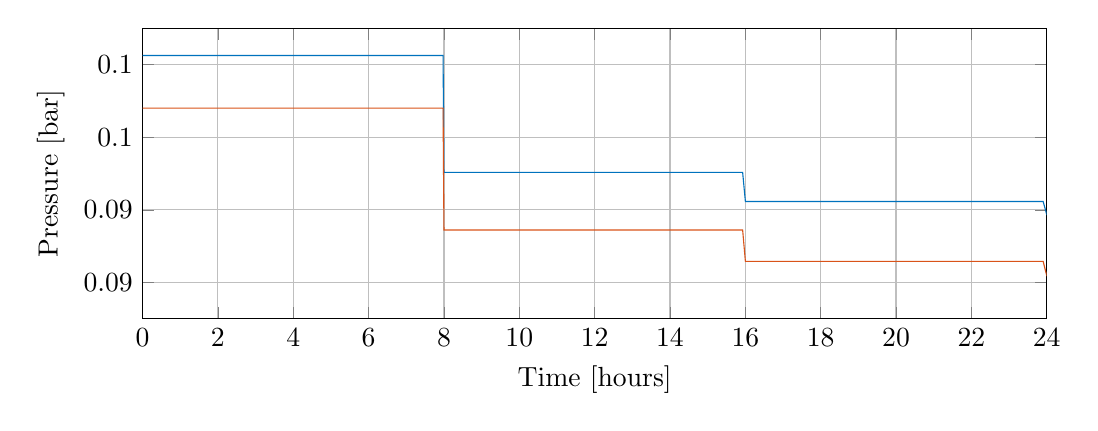
\begin{tikzpicture}

\begin{axis}[%
scaled y ticks = false,
 y tick label style={/pgf/number format/fixed,
/pgf/number format/1000 sep = \thinspace}, % Optional if you want to replace comma as the 1000 separator
width=4.521in,
height=1.453in,
at={(1.011in,0.642in)},
scale only axis,
xmin=0,
xmax=24,
xlabel={Time [hours]},
xmajorgrids,
ymin=0.091,
ymax=0.099,
ylabel={Pressure [bar]},
ymajorgrids,
axis background/.style={fill=white}
]
\addplot [color=mycolor1,solid,forget plot]
  table[row sep=crcr]{%
0	0.098247686329957\\
0.340448888888889	0.098247686329957\\
0.680897777777778	0.098247686329957\\
0.997028888888889	0.098247686329957\\
1.33747777777778	0.098247686329957\\
1.67792666666667	0.098247686329957\\
1.99405777777778	0.098247686329957\\
2.33450666666667	0.098247686329957\\
2.67495555555556	0.098247686329957\\
2.99108666666667	0.098247686329957\\
3.33153555555556	0.098247686329957\\
3.67198444444444	0.098247686329957\\
3.98811555555556	0.098247686329957\\
4.32856444444444	0.098247686329957\\
4.66901333333333	0.098247686329957\\
4.98514444444444	0.098247686329957\\
5.32559333333333	0.098247686329957\\
5.64172444444444	0.098247686329957\\
5.98217333333333	0.098247686329957\\
6.32262222222222	0.098247686329957\\
6.63875333333333	0.098247686329957\\
6.97920222222222	0.098247686329957\\
7.31965111111111	0.098247686329957\\
7.63578222222222	0.098247686329957\\
7.97623111111111	0.098247686329957\\
8.00054888888889	0.0950314633261829\\
8.31668	0.0950314633261829\\
8.63281111111111	0.0950314633261829\\
8.97326	0.0950314633261829\\
9.31370888888889	0.0950314633261829\\
9.62984	0.0950314633261829\\
9.97028888888889	0.0950314633261829\\
10.28642	0.0950314633261829\\
10.6268688888889	0.0950314633261829\\
10.9673177777778	0.0950314633261829\\
11.2834488888889	0.0950314633261829\\
11.6238977777778	0.0950314633261829\\
11.9643466666667	0.0950314633261829\\
12.2804777777778	0.0950314633261829\\
12.6209266666667	0.0950314633261829\\
12.9613755555556	0.0950314633261829\\
13.2775066666667	0.0950314633261829\\
13.6179555555556	0.0950314633261829\\
13.9340866666667	0.0950314633261829\\
14.2745355555556	0.0950314633261829\\
14.6149844444444	0.0950314633261829\\
14.9311155555556	0.0950314633261829\\
15.2715644444444	0.0950314633261829\\
15.6120133333333	0.0950314633261829\\
15.9281444444444	0.0950314633261829\\
16.0010977777778	0.0942300382577624\\
16.2685933333333	0.0942300382577624\\
16.6090422222222	0.0942300382577624\\
16.9251733333333	0.0942300382577624\\
17.2656222222222	0.0942300382577624\\
17.6060711111111	0.0942300382577624\\
17.9222022222222	0.0942300382577624\\
18.2626511111111	0.0942300382577624\\
18.6031	0.0942300382577624\\
18.9192311111111	0.0942300382577624\\
19.25968	0.0942300382577624\\
19.5758111111111	0.0942300382577624\\
19.91626	0.0942300382577624\\
20.2567088888889	0.0942300382577624\\
20.57284	0.0942300382577624\\
20.9132888888889	0.0942300382577624\\
21.2537377777778	0.0942300382577624\\
21.5698688888889	0.0942300382577624\\
21.9103177777778	0.0942300382577624\\
22.2507666666667	0.0942300382577624\\
22.5668977777778	0.0942300382577624\\
22.9073466666667	0.0942300382577624\\
23.2234777777778	0.0942300382577624\\
23.5639266666667	0.0942300382577624\\
23.9043755555556	0.0942300382577624\\
24.0016466666667	0.09386457857937\\
24.2205066666667	0.09386457857937\\
24.5609555555556	0.09386457857937\\
24.9014044444444	0.09386457857937\\
25.2175355555556	0.09386457857937\\
25.5579844444444	0.09386457857937\\
25.8984333333333	0.09386457857937\\
26.2145644444444	0.09386457857937\\
26.5550133333333	0.09386457857937\\
26.8954622222222	0.09386457857937\\
27.2115933333333	0.09386457857937\\
27.5520422222222	0.09386457857937\\
27.8681733333333	0.09386457857937\\
28.2086222222222	0.09386457857937\\
28.5490711111111	0.09386457857937\\
28.8652022222222	0.09386457857937\\
29.2056511111111	0.09386457857937\\
29.5461	0.09386457857937\\
29.8622311111111	0.09386457857937\\
30.20268	0.09386457857937\\
30.5431288888889	0.09386457857937\\
30.85926	0.09386457857937\\
31.1997088888889	0.09386457857937\\
31.5401577777778	0.09386457857937\\
31.8562888888889	0.09386457857937\\
32.1967377777778	0.09386457857937\\
32.5128688888889	0.09386457857937\\
32.8533177777778	0.09386457857937\\
33.1937666666667	0.09386457857937\\
33.5098977777778	0.09386457857937\\
33.8503466666667	0.09386457857937\\
34.1907955555556	0.09386457857937\\
34.5069266666667	0.09386457857937\\
34.8473755555556	0.09386457857937\\
35.1878244444444	0.09386457857937\\
35.5039555555555	0.09386457857937\\
35.8444044444444	0.09386457857937\\
36.1848533333333	0.09386457857937\\
36.5009844444444	0.09386457857937\\
36.8414333333333	0.09386457857937\\
37.1818822222222	0.09386457857937\\
37.4980133333333	0.09386457857937\\
37.8384622222222	0.09386457857937\\
38.1545933333333	0.09386457857937\\
38.4950422222222	0.09386457857937\\
38.8354911111111	0.09386457857937\\
39.1516222222222	0.09386457857937\\
39.4920711111111	0.09386457857937\\
39.83252	0.09386457857937\\
40.1486511111111	0.09386457857937\\
40.4891	0.09386457857937\\
40.8295488888889	0.09386457857937\\
41.14568	0.09386457857937\\
41.4861288888889	0.09386457857937\\
41.8265777777778	0.09386457857937\\
42.1427088888889	0.09386457857937\\
42.4831577777778	0.09386457857937\\
42.7992888888889	0.09386457857937\\
43.1397377777778	0.09386457857937\\
43.4801866666667	0.09386457857937\\
43.7963177777778	0.09386457857937\\
44.1367666666667	0.09386457857937\\
44.4772155555556	0.09386457857937\\
44.7933466666667	0.09386457857937\\
45.1337955555556	0.09386457857937\\
45.4742444444444	0.09386457857937\\
45.7903755555555	0.09386457857937\\
46.1308244444444	0.09386457857937\\
46.4469555555556	0.09386457857937\\
46.7874044444444	0.09386457857937\\
47.1278533333333	0.09386457857937\\
47.4439844444444	0.09386457857937\\
47.7844333333333	0.09386457857937\\
48.1248822222222	0.09386457857937\\
48.4410133333333	0.09386457857937\\
48.7814622222222	0.09386457857937\\
49.0003222222222	0.0938856977625195\\
49.1219111111111	0.0938856977625195\\
49.4380422222222	0.0938856977625195\\
49.7784911111111	0.0938856977625195\\
50.11894	0.0938856977625195\\
50.4350711111111	0.0938856977625195\\
50.77552	0.0938856977625195\\
51.1159688888889	0.0938856977625195\\
51.4321	0.0938856977625195\\
51.7725488888889	0.0938856977625195\\
52.08868	0.0938856977625195\\
52.4291288888889	0.0938856977625195\\
52.7695777777778	0.0938856977625195\\
53.0857088888889	0.0938856977625195\\
53.4261577777778	0.0938856977625195\\
53.7666066666667	0.0938856977625195\\
54.0827377777778	0.0938856977625195\\
54.4231866666667	0.0938856977625195\\
54.7636355555556	0.0938856977625195\\
55.0797666666667	0.0938856977625195\\
55.4202155555556	0.0938856977625195\\
55.7363466666667	0.0938856977625195\\
56.0767955555556	0.0938856977625195\\
56.4172444444444	0.0938856977625195\\
56.7333755555556	0.0938856977625195\\
57.0008711111111	0.0946758041347748\\
57.0738244444444	0.0946758041347748\\
57.4142733333333	0.0946758041347748\\
57.7304044444444	0.0946758041347748\\
58.0708533333333	0.0946758041347748\\
58.4113022222222	0.0946758041347748\\
58.7274333333333	0.0946758041347748\\
59.0678822222222	0.0946758041347748\\
59.4083311111111	0.0946758041347748\\
59.7244622222222	0.0946758041347748\\
60.0649111111111	0.0946758041347748\\
60.40536	0.0946758041347748\\
60.7214911111111	0.0946758041347748\\
61.06194	0.0946758041347748\\
61.3780711111111	0.0946758041347748\\
61.71852	0.0946758041347748\\
62.0589688888889	0.0946758041347748\\
62.3751	0.0946758041347748\\
62.7155488888889	0.0946758041347748\\
63.0559977777778	0.0946758041347748\\
63.3721288888889	0.0946758041347748\\
63.7125777777778	0.0946758041347748\\
64.0530266666667	0.0946758041347748\\
64.3691577777778	0.0946758041347748\\
64.7096066666667	0.0946758041347748\\
65.00142	0.0943943146847119\\
65.0257377777778	0.0943943146847119\\
65.3661866666667	0.0943943146847119\\
65.7066355555556	0.0943943146847119\\
66.0227666666667	0.0943943146847119\\
66.3632155555556	0.0943943146847119\\
66.7036644444444	0.0943943146847119\\
67.0197955555556	0.0943943146847119\\
67.3602444444444	0.0943943146847119\\
67.7006933333333	0.0943943146847119\\
68.0168244444444	0.0943943146847119\\
68.3572733333333	0.0943943146847119\\
68.6977222222222	0.0943943146847119\\
69.0138533333333	0.0943943146847119\\
69.3543022222222	0.0943943146847119\\
69.6704333333333	0.0943943146847119\\
70.0108822222222	0.0943943146847119\\
70.3513311111111	0.0943943146847119\\
70.6674622222222	0.0943943146847119\\
71.0079111111111	0.0943943146847119\\
71.34836	0.0943943146847119\\
71.6644911111111	0.0943943146847119\\
72.00494	0.0943943146847119\\
72.3453888888889	0.0943943146847119\\
72.66152	0.0943943146847119\\
73.0019688888889	0.0943943146847119\\
73.3424177777778	0.0943943146847119\\
73.6585488888889	0.0943943146847119\\
73.9989977777778	0.0943943146847119\\
74.3394466666667	0.0943943146847119\\
74.6555777777778	0.0943943146847119\\
74.9960266666667	0.0943943146847119\\
75.3121577777778	0.0943943146847119\\
75.6526066666667	0.0943943146847119\\
75.9930555555556	0.0943943146847119\\
76.3091866666667	0.0943943146847119\\
76.6496355555555	0.0943943146847119\\
76.9900844444444	0.0943943146847119\\
77.3062155555556	0.0943943146847119\\
77.6466644444444	0.0943943146847119\\
77.9871133333333	0.0943943146847119\\
78.3032444444444	0.0943943146847119\\
78.6436933333333	0.0943943146847119\\
78.9598244444445	0.0943943146847119\\
79.3002733333333	0.0943943146847119\\
79.6407222222222	0.0943943146847119\\
79.9568533333333	0.0943943146847119\\
80.2973022222222	0.0943943146847119\\
80.6377511111111	0.0943943146847119\\
80.9538822222222	0.0943943146847119\\
81.2943311111111	0.0943943146847119\\
81.63478	0.0943943146847119\\
81.9509111111111	0.0943943146847119\\
82.29136	0.0943943146847119\\
82.6318088888889	0.0943943146847119\\
82.94794	0.0943943146847119\\
83.2883888888889	0.0943943146847119\\
83.6288377777778	0.0943943146847119\\
83.9449688888889	0.0943943146847119\\
84.2854177777778	0.0943943146847119\\
84.6015488888889	0.0943943146847119\\
84.9419977777778	0.0943943146847119\\
85.2824466666667	0.0943943146847119\\
85.5985777777778	0.0943943146847119\\
85.9390266666667	0.0943943146847119\\
86.2794755555555	0.0943943146847119\\
86.5956066666667	0.0943943146847119\\
86.9360555555556	0.0943943146847119\\
87.2765044444444	0.0943943146847119\\
87.5926355555556	0.0943943146847119\\
87.9330844444444	0.0943943146847119\\
88.2735333333333	0.0943943146847119\\
88.5896644444445	0.0943943146847119\\
88.9301133333333	0.0943943146847119\\
89.2462444444444	0.0943943146847119\\
89.5866933333333	0.0943943146847119\\
89.9271422222222	0.0943943146847119\\
90.0000955555555	0.094544338146617\\
90.2432733333333	0.094544338146617\\
90.5837222222222	0.094544338146617\\
90.9241711111111	0.094544338146617\\
91.2403022222222	0.094544338146617\\
91.5807511111111	0.094544338146617\\
91.9212	0.094544338146617\\
92.2373311111111	0.094544338146617\\
92.57778	0.094544338146617\\
92.8939111111111	0.094544338146617\\
93.23436	0.094544338146617\\
93.5748088888889	0.094544338146617\\
93.89094	0.094544338146617\\
94.2313888888889	0.094544338146617\\
94.5718377777778	0.094544338146617\\
94.8879688888889	0.094544338146617\\
95.2284177777778	0.094544338146617\\
95.5688666666667	0.094544338146617\\
95.8849977777778	0.094544338146617\\
96.2254466666667	0.094544338146617\\
96.5658955555556	0.094544338146617\\
96.8820266666667	0.094544338146617\\
97.2224755555556	0.094544338146617\\
97.5386066666667	0.094544338146617\\
97.8790555555556	0.094544338146617\\
98.0006444444444	0.0935709811972999\\
98.2195044444445	0.0935709811972999\\
98.5356355555556	0.0935709811972999\\
98.8760844444444	0.0935709811972999\\
99.2165333333333	0.0935709811972999\\
99.5326644444444	0.0935709811972999\\
99.8731133333333	0.0935709811972999\\
100.213562222222	0.0935709811972999\\
100.529693333333	0.0935709811972999\\
100.870142222222	0.0935709811972999\\
101.210591111111	0.0935709811972999\\
101.526722222222	0.0935709811972999\\
101.867171111111	0.0935709811972999\\
102.20762	0.0935709811972999\\
102.523751111111	0.0935709811972999\\
102.8642	0.0935709811972999\\
103.180331111111	0.0935709811972999\\
103.52078	0.0935709811972999\\
103.861228888889	0.0935709811972999\\
104.17736	0.0935709811972999\\
104.517808888889	0.0935709811972999\\
104.858257777778	0.0935709811972999\\
105.174388888889	0.0935709811972999\\
105.514837777778	0.0935709811972999\\
105.855286666667	0.0935709811972999\\
106.001193333333	0.0948578188143902\\
106.171417777778	0.0948578188143902\\
106.511866666667	0.0948578188143902\\
106.852315555556	0.0948578188143902\\
107.168446666667	0.0948578188143902\\
107.508895555556	0.0948578188143902\\
107.825026666667	0.0948578188143902\\
108.165475555556	0.0948578188143902\\
108.505924444444	0.0948578188143902\\
108.822055555556	0.0948578188143902\\
109.162504444444	0.0948578188143902\\
109.502953333333	0.0948578188143902\\
109.819084444444	0.0948578188143902\\
110.159533333333	0.0948578188143902\\
110.499982222222	0.0948578188143902\\
110.816113333333	0.0948578188143902\\
111.156562222222	0.0948578188143902\\
111.472693333333	0.0948578188143902\\
111.813142222222	0.0948578188143902\\
112.153591111111	0.0948578188143902\\
112.469722222222	0.0948578188143902\\
112.810171111111	0.0948578188143902\\
113.15062	0.0948578188143902\\
113.466751111111	0.0948578188143902\\
113.8072	0.0948578188143902\\
114.001742222222	0.0947164591471082\\
114.147648888889	0.0947164591471082\\
114.46378	0.0947164591471082\\
114.804228888889	0.0947164591471082\\
115.144677777778	0.0947164591471082\\
115.460808888889	0.0947164591471082\\
115.801257777778	0.0947164591471082\\
116.141706666667	0.0947164591471082\\
116.457837777778	0.0947164591471082\\
116.798286666667	0.0947164591471082\\
117.114417777778	0.0947164591471082\\
117.454866666667	0.0947164591471082\\
117.795315555556	0.0947164591471082\\
118.111446666667	0.0947164591471082\\
118.451895555556	0.0947164591471082\\
118.792344444444	0.0947164591471082\\
119.108475555556	0.0947164591471082\\
119.448924444444	0.0947164591471082\\
119.789373333333	0.0947164591471082\\
120.105504444444	0.0947164591471082\\
120.445953333333	0.0947164591471082\\
120.786402222222	0.0947164591471082\\
121.102533333333	0.0947164591471082\\
121.442982222222	0.0947164591471082\\
121.759113333333	0.0947164591471082\\
122.099562222222	0.0947164591471082\\
122.440011111111	0.0947164591471082\\
122.756142222222	0.0947164591471082\\
123.096591111111	0.0947164591471082\\
123.43704	0.0947164591471082\\
123.753171111111	0.0947164591471082\\
124.09362	0.0947164591471082\\
124.434068888889	0.0947164591471082\\
124.7502	0.0947164591471082\\
125.090648888889	0.0947164591471082\\
125.431097777778	0.0947164591471082\\
125.747228888889	0.0947164591471082\\
126.087677777778	0.0947164591471082\\
126.403808888889	0.0947164591471082\\
126.744257777778	0.0947164591471082\\
127.084706666667	0.0947164591471082\\
127.400837777778	0.0947164591471082\\
127.741286666667	0.0947164591471082\\
128.081735555556	0.0947164591471082\\
128.397866666667	0.0947164591471082\\
128.738315555556	0.0947164591471082\\
129.078764444444	0.0947164591471082\\
129.394895555556	0.0947164591471082\\
129.735344444444	0.0947164591471082\\
130.051475555556	0.0947164591471082\\
130.391924444444	0.0947164591471082\\
130.732373333333	0.0947164591471082\\
131.048504444444	0.0947164591471082\\
131.388953333333	0.0947164591471082\\
131.729402222222	0.0947164591471082\\
132.045533333333	0.0947164591471082\\
132.385982222222	0.0947164591471082\\
132.726431111111	0.0947164591471082\\
133.042562222222	0.0947164591471082\\
133.383011111111	0.0947164591471082\\
133.72346	0.0947164591471082\\
134.039591111111	0.0947164591471082\\
134.38004	0.0947164591471082\\
134.696171111111	0.0947164591471082\\
135.03662	0.0947164591471082\\
135.377068888889	0.0947164591471082\\
135.6932	0.0947164591471082\\
136.033648888889	0.0947164591471082\\
136.374097777778	0.0947164591471082\\
136.690228888889	0.0947164591471082\\
137.030677777778	0.0947164591471082\\
137.371126666667	0.0947164591471082\\
137.687257777778	0.0947164591471082\\
138.027706666667	0.0947164591471082\\
138.368155555556	0.0947164591471082\\
138.684286666667	0.0947164591471082\\
139.000417777778	0.0950439603825615\\
139.024735555556	0.0950439603825615\\
139.340866666667	0.0950439603825615\\
139.681315555556	0.0950439603825615\\
140.021764444444	0.0950439603825615\\
140.337895555556	0.0950439603825615\\
140.678344444444	0.0950439603825615\\
141.018793333333	0.0950439603825615\\
141.334924444444	0.0950439603825615\\
141.675373333333	0.0950439603825615\\
142.015822222222	0.0950439603825615\\
142.331953333333	0.0950439603825615\\
142.672402222222	0.0950439603825615\\
143.012851111111	0.0950439603825615\\
143.328982222222	0.0950439603825615\\
143.985562222222	0.0950439603825615\\
};
\addplot [color=mycolor2,solid,forget plot]
  table[row sep=crcr]{%
0	0.0967984845464634\\
0.340448888888889	0.0967984845464634\\
0.680897777777778	0.0967984845464634\\
0.997028888888889	0.0967984845464634\\
1.33747777777778	0.0967984845464634\\
1.67792666666667	0.0967984845464634\\
1.99405777777778	0.0967984845464634\\
2.33450666666667	0.0967984845464634\\
2.67495555555556	0.0967984845464634\\
2.99108666666667	0.0967984845464634\\
3.33153555555556	0.0967984845464634\\
3.67198444444444	0.0967984845464634\\
3.98811555555556	0.0967984845464634\\
4.32856444444444	0.0967984845464634\\
4.66901333333333	0.0967984845464634\\
4.98514444444444	0.0967984845464634\\
5.32559333333333	0.0967984845464634\\
5.64172444444444	0.0967984845464634\\
5.98217333333333	0.0967984845464634\\
6.32262222222222	0.0967984845464634\\
6.63875333333333	0.0967984845464634\\
6.97920222222222	0.0967984845464634\\
7.31965111111111	0.0967984845464634\\
7.63578222222222	0.0967984845464634\\
7.97623111111111	0.0967984845464634\\
8.00054888888889	0.0934450210155314\\
8.31668	0.0934450210155314\\
8.63281111111111	0.0934450210155314\\
8.97326	0.0934450210155314\\
9.31370888888889	0.0934450210155314\\
9.62984	0.0934450210155314\\
9.97028888888889	0.0934450210155314\\
10.28642	0.0934450210155314\\
10.6268688888889	0.0934450210155314\\
10.9673177777778	0.0934450210155314\\
11.2834488888889	0.0934450210155314\\
11.6238977777778	0.0934450210155314\\
11.9643466666667	0.0934450210155314\\
12.2804777777778	0.0934450210155314\\
12.6209266666667	0.0934450210155314\\
12.9613755555556	0.0934450210155314\\
13.2775066666667	0.0934450210155314\\
13.6179555555556	0.0934450210155314\\
13.9340866666667	0.0934450210155314\\
14.2745355555556	0.0934450210155314\\
14.6149844444444	0.0934450210155314\\
14.9311155555556	0.0934450210155314\\
15.2715644444444	0.0934450210155314\\
15.6120133333333	0.0934450210155314\\
15.9281444444444	0.0934450210155314\\
16.0010977777778	0.092582311295702\\
16.2685933333333	0.092582311295702\\
16.6090422222222	0.092582311295702\\
16.9251733333333	0.092582311295702\\
17.2656222222222	0.092582311295702\\
17.6060711111111	0.092582311295702\\
17.9222022222222	0.092582311295702\\
18.2626511111111	0.092582311295702\\
18.6031	0.092582311295702\\
18.9192311111111	0.092582311295702\\
19.25968	0.092582311295702\\
19.5758111111111	0.092582311295702\\
19.91626	0.092582311295702\\
20.2567088888889	0.092582311295702\\
20.57284	0.092582311295702\\
20.9132888888889	0.092582311295702\\
21.2537377777778	0.092582311295702\\
21.5698688888889	0.092582311295702\\
21.9103177777778	0.092582311295702\\
22.2507666666667	0.092582311295702\\
22.5668977777778	0.092582311295702\\
22.9073466666667	0.092582311295702\\
23.2234777777778	0.092582311295702\\
23.5639266666667	0.092582311295702\\
23.9043755555556	0.092582311295702\\
24.0016466666667	0.0921803662430968\\
24.2205066666667	0.0921803662430968\\
24.5609555555556	0.0921803662430968\\
24.9014044444444	0.0921803662430968\\
25.2175355555556	0.0921803662430968\\
25.5579844444444	0.0921803662430968\\
25.8984333333333	0.0921803662430968\\
26.2145644444444	0.0921803662430968\\
26.5550133333333	0.0921803662430968\\
26.8954622222222	0.0921803662430968\\
27.2115933333333	0.0921803662430968\\
27.5520422222222	0.0921803662430968\\
27.8681733333333	0.0921803662430968\\
28.2086222222222	0.0921803662430968\\
28.5490711111111	0.0921803662430968\\
28.8652022222222	0.0921803662430968\\
29.2056511111111	0.0921803662430968\\
29.5461	0.0921803662430968\\
29.8622311111111	0.0921803662430968\\
30.20268	0.0921803662430968\\
30.5431288888889	0.0921803662430968\\
30.85926	0.0921803662430968\\
31.1997088888889	0.0921803662430968\\
31.5401577777778	0.0921803662430968\\
31.8562888888889	0.0921803662430968\\
32.1967377777778	0.0921803662430968\\
32.5128688888889	0.0921803662430968\\
32.8533177777778	0.0921803662430968\\
33.1937666666667	0.0921803662430968\\
33.5098977777778	0.0921803662430968\\
33.8503466666667	0.0921803662430968\\
34.1907955555556	0.0921803662430968\\
34.5069266666667	0.0921803662430968\\
34.8473755555556	0.0921803662430968\\
35.1878244444444	0.0921803662430968\\
35.5039555555555	0.0921803662430968\\
35.8444044444444	0.0921803662430968\\
36.1848533333333	0.0921803662430968\\
36.5009844444444	0.0921803662430968\\
36.8414333333333	0.0921803662430968\\
37.1818822222222	0.0921803662430968\\
37.4980133333333	0.0921803662430968\\
37.8384622222222	0.0921803662430968\\
38.1545933333333	0.0921803662430968\\
38.4950422222222	0.0921803662430968\\
38.8354911111111	0.0921803662430968\\
39.1516222222222	0.0921803662430968\\
39.4920711111111	0.0921803662430968\\
39.83252	0.0921803662430968\\
40.1486511111111	0.0921803662430968\\
40.4891	0.0921803662430968\\
40.8295488888889	0.0921803662430968\\
41.14568	0.0921803662430968\\
41.4861288888889	0.0921803662430968\\
41.8265777777778	0.0921803662430968\\
42.1427088888889	0.0921803662430968\\
42.4831577777778	0.0921803662430968\\
42.7992888888889	0.0921803662430968\\
43.1397377777778	0.0921803662430968\\
43.4801866666667	0.0921803662430968\\
43.7963177777778	0.0921803662430968\\
44.1367666666667	0.0921803662430968\\
44.4772155555556	0.0921803662430968\\
44.7933466666667	0.0921803662430968\\
45.1337955555556	0.0921803662430968\\
45.4742444444444	0.0921803662430968\\
45.7903755555555	0.0921803662430968\\
46.1308244444444	0.0921803662430968\\
46.4469555555556	0.0921803662430968\\
46.7874044444444	0.0921803662430968\\
47.1278533333333	0.0921803662430968\\
47.4439844444444	0.0921803662430968\\
47.7844333333333	0.0921803662430968\\
48.1248822222222	0.0921803662430968\\
48.4410133333333	0.0921803662430968\\
48.7814622222222	0.0921803662430968\\
49.0003222222222	0.0922054477835333\\
49.1219111111111	0.0922054477835333\\
49.4380422222222	0.0922054477835333\\
49.7784911111111	0.0922054477835333\\
50.11894	0.0922054477835333\\
50.4350711111111	0.0922054477835333\\
50.77552	0.0922054477835333\\
51.1159688888889	0.0922054477835333\\
51.4321	0.0922054477835333\\
51.7725488888889	0.0922054477835333\\
52.08868	0.0922054477835333\\
52.4291288888889	0.0922054477835333\\
52.7695777777778	0.0922054477835333\\
53.0857088888889	0.0922054477835333\\
53.4261577777778	0.0922054477835333\\
53.7666066666667	0.0922054477835333\\
54.0827377777778	0.0922054477835333\\
54.4231866666667	0.0922054477835333\\
54.7636355555556	0.0922054477835333\\
55.0797666666667	0.0922054477835333\\
55.4202155555556	0.0922054477835333\\
55.7363466666667	0.0922054477835333\\
56.0767955555556	0.0922054477835333\\
56.4172444444444	0.0922054477835333\\
56.7333755555556	0.0922054477835333\\
57.0008711111111	0.0930556940674386\\
57.0738244444444	0.0930556940674386\\
57.4142733333333	0.0930556940674386\\
57.7304044444444	0.0930556940674386\\
58.0708533333333	0.0930556940674386\\
58.4113022222222	0.0930556940674386\\
58.7274333333333	0.0930556940674386\\
59.0678822222222	0.0930556940674386\\
59.4083311111111	0.0930556940674386\\
59.7244622222222	0.0930556940674386\\
60.0649111111111	0.0930556940674386\\
60.40536	0.0930556940674386\\
60.7214911111111	0.0930556940674386\\
61.06194	0.0930556940674386\\
61.3780711111111	0.0930556940674386\\
61.71852	0.0930556940674386\\
62.0589688888889	0.0930556940674386\\
62.3751	0.0930556940674386\\
62.7155488888889	0.0930556940674386\\
63.0559977777778	0.0930556940674386\\
63.3721288888889	0.0930556940674386\\
63.7125777777778	0.0930556940674386\\
64.0530266666667	0.0930556940674386\\
64.3691577777778	0.0930556940674386\\
64.7096066666667	0.0930556940674386\\
65.00142	0.0928086801922649\\
65.0257377777778	0.0928086801922649\\
65.3661866666667	0.0928086801922649\\
65.7066355555556	0.0928086801922649\\
66.0227666666667	0.0928086801922649\\
66.3632155555556	0.0928086801922649\\
66.7036644444444	0.0928086801922649\\
67.0197955555556	0.0928086801922649\\
67.3602444444444	0.0928086801922649\\
67.7006933333333	0.0928086801922649\\
68.0168244444444	0.0928086801922649\\
68.3572733333333	0.0928086801922649\\
68.6977222222222	0.0928086801922649\\
69.0138533333333	0.0928086801922649\\
69.3543022222222	0.0928086801922649\\
69.6704333333333	0.0928086801922649\\
70.0108822222222	0.0928086801922649\\
70.3513311111111	0.0928086801922649\\
70.6674622222222	0.0928086801922649\\
71.0079111111111	0.0928086801922649\\
71.34836	0.0928086801922649\\
71.6644911111111	0.0928086801922649\\
72.00494	0.0928086801922649\\
72.3453888888889	0.0928086801922649\\
72.66152	0.0928086801922649\\
73.0019688888889	0.0928086801922649\\
73.3424177777778	0.0928086801922649\\
73.6585488888889	0.0928086801922649\\
73.9989977777778	0.0928086801922649\\
74.3394466666667	0.0928086801922649\\
74.6555777777778	0.0928086801922649\\
74.9960266666667	0.0928086801922649\\
75.3121577777778	0.0928086801922649\\
75.6526066666667	0.0928086801922649\\
75.9930555555556	0.0928086801922649\\
76.3091866666667	0.0928086801922649\\
76.6496355555555	0.0928086801922649\\
76.9900844444444	0.0928086801922649\\
77.3062155555556	0.0928086801922649\\
77.6466644444444	0.0928086801922649\\
77.9871133333333	0.0928086801922649\\
78.3032444444444	0.0928086801922649\\
78.6436933333333	0.0928086801922649\\
78.9598244444445	0.0928086801922649\\
79.3002733333333	0.0928086801922649\\
79.6407222222222	0.0928086801922649\\
79.9568533333333	0.0928086801922649\\
80.2973022222222	0.0928086801922649\\
80.6377511111111	0.0928086801922649\\
80.9538822222222	0.0928086801922649\\
81.2943311111111	0.0928086801922649\\
81.63478	0.0928086801922649\\
81.9509111111111	0.0928086801922649\\
82.29136	0.0928086801922649\\
82.6318088888889	0.0928086801922649\\
82.94794	0.0928086801922649\\
83.2883888888889	0.0928086801922649\\
83.6288377777778	0.0928086801922649\\
83.9449688888889	0.0928086801922649\\
84.2854177777778	0.0928086801922649\\
84.6015488888889	0.0928086801922649\\
84.9419977777778	0.0928086801922649\\
85.2824466666667	0.0928086801922649\\
85.5985777777778	0.0928086801922649\\
85.9390266666667	0.0928086801922649\\
86.2794755555555	0.0928086801922649\\
86.5956066666667	0.0928086801922649\\
86.9360555555556	0.0928086801922649\\
87.2765044444444	0.0928086801922649\\
87.5926355555556	0.0928086801922649\\
87.9330844444444	0.0928086801922649\\
88.2735333333333	0.0928086801922649\\
88.5896644444445	0.0928086801922649\\
88.9301133333333	0.0928086801922649\\
89.2462444444444	0.0928086801922649\\
89.5866933333333	0.0928086801922649\\
89.9271422222222	0.0928086801922649\\
90.0000955555555	0.0929232434539679\\
90.2432733333333	0.0929232434539679\\
90.5837222222222	0.0929232434539679\\
90.9241711111111	0.0929232434539679\\
91.2403022222222	0.0929232434539679\\
91.5807511111111	0.0929232434539679\\
91.9212	0.0929232434539679\\
92.2373311111111	0.0929232434539679\\
92.57778	0.0929232434539679\\
92.8939111111111	0.0929232434539679\\
93.23436	0.0929232434539679\\
93.5748088888889	0.0929232434539679\\
93.89094	0.0929232434539679\\
94.2313888888889	0.0929232434539679\\
94.5718377777778	0.0929232434539679\\
94.8879688888889	0.0929232434539679\\
95.2284177777778	0.0929232434539679\\
95.5688666666667	0.0929232434539679\\
95.8849977777778	0.0929232434539679\\
96.2254466666667	0.0929232434539679\\
96.5658955555556	0.0929232434539679\\
96.8820266666667	0.0929232434539679\\
97.2224755555556	0.0929232434539679\\
97.5386066666667	0.0929232434539679\\
97.8790555555556	0.0929232434539679\\
98.0006444444444	0.0918610855339023\\
98.2195044444445	0.0918610855339023\\
98.5356355555556	0.0918610855339023\\
98.8760844444444	0.0918610855339023\\
99.2165333333333	0.0918610855339023\\
99.5326644444444	0.0918610855339023\\
99.8731133333333	0.0918610855339023\\
100.213562222222	0.0918610855339023\\
100.529693333333	0.0918610855339023\\
100.870142222222	0.0918610855339023\\
101.210591111111	0.0918610855339023\\
101.526722222222	0.0918610855339023\\
101.867171111111	0.0918610855339023\\
102.20762	0.0918610855339023\\
102.523751111111	0.0918610855339023\\
102.8642	0.0918610855339023\\
103.180331111111	0.0918610855339023\\
103.52078	0.0918610855339023\\
103.861228888889	0.0918610855339023\\
104.17736	0.0918610855339023\\
104.517808888889	0.0918610855339023\\
104.858257777778	0.0918610855339023\\
105.174388888889	0.0918610855339023\\
105.514837777778	0.0918610855339023\\
105.855286666667	0.0918610855339023\\
106.001193333333	0.093245427660319\\
106.171417777778	0.093245427660319\\
106.511866666667	0.093245427660319\\
106.852315555556	0.093245427660319\\
107.168446666667	0.093245427660319\\
107.508895555556	0.093245427660319\\
107.825026666667	0.093245427660319\\
108.165475555556	0.093245427660319\\
108.505924444444	0.093245427660319\\
108.822055555556	0.093245427660319\\
109.162504444444	0.093245427660319\\
109.502953333333	0.093245427660319\\
109.819084444444	0.093245427660319\\
110.159533333333	0.093245427660319\\
110.499982222222	0.093245427660319\\
110.816113333333	0.093245427660319\\
111.156562222222	0.093245427660319\\
111.472693333333	0.093245427660319\\
111.813142222222	0.093245427660319\\
112.153591111111	0.093245427660319\\
112.469722222222	0.093245427660319\\
112.810171111111	0.093245427660319\\
113.15062	0.093245427660319\\
113.466751111111	0.093245427660319\\
113.8072	0.093245427660319\\
114.001742222222	0.0930982634358413\\
114.147648888889	0.0930982634358413\\
114.46378	0.0930982634358413\\
114.804228888889	0.0930982634358413\\
115.144677777778	0.0930982634358413\\
115.460808888889	0.0930982634358413\\
115.801257777778	0.0930982634358413\\
116.141706666667	0.0930982634358413\\
116.457837777778	0.0930982634358413\\
116.798286666667	0.0930982634358413\\
117.114417777778	0.0930982634358413\\
117.454866666667	0.0930982634358413\\
117.795315555556	0.0930982634358413\\
118.111446666667	0.0930982634358413\\
118.451895555556	0.0930982634358413\\
118.792344444444	0.0930982634358413\\
119.108475555556	0.0930982634358413\\
119.448924444444	0.0930982634358413\\
119.789373333333	0.0930982634358413\\
120.105504444444	0.0930982634358413\\
120.445953333333	0.0930982634358413\\
120.786402222222	0.0930982634358413\\
121.102533333333	0.0930982634358413\\
121.442982222222	0.0930982634358413\\
121.759113333333	0.0930982634358413\\
122.099562222222	0.0930982634358413\\
122.440011111111	0.0930982634358413\\
122.756142222222	0.0930982634358413\\
123.096591111111	0.0930982634358413\\
123.43704	0.0930982634358413\\
123.753171111111	0.0930982634358413\\
124.09362	0.0930982634358413\\
124.434068888889	0.0930982634358413\\
124.7502	0.0930982634358413\\
125.090648888889	0.0930982634358413\\
125.431097777778	0.0930982634358413\\
125.747228888889	0.0930982634358413\\
126.087677777778	0.0930982634358413\\
126.403808888889	0.0930982634358413\\
126.744257777778	0.0930982634358413\\
127.084706666667	0.0930982634358413\\
127.400837777778	0.0930982634358413\\
127.741286666667	0.0930982634358413\\
128.081735555556	0.0930982634358413\\
128.397866666667	0.0930982634358413\\
128.738315555556	0.0930982634358413\\
129.078764444444	0.0930982634358413\\
129.394895555556	0.0930982634358413\\
129.735344444444	0.0930982634358413\\
130.051475555556	0.0930982634358413\\
130.391924444444	0.0930982634358413\\
130.732373333333	0.0930982634358413\\
131.048504444444	0.0930982634358413\\
131.388953333333	0.0930982634358413\\
131.729402222222	0.0930982634358413\\
132.045533333333	0.0930982634358413\\
132.385982222222	0.0930982634358413\\
132.726431111111	0.0930982634358413\\
133.042562222222	0.0930982634358413\\
133.383011111111	0.0930982634358413\\
133.72346	0.0930982634358413\\
134.039591111111	0.0930982634358413\\
134.38004	0.0930982634358413\\
134.696171111111	0.0930982634358413\\
135.03662	0.0930982634358413\\
135.377068888889	0.0930982634358413\\
135.6932	0.0930982634358413\\
136.033648888889	0.0930982634358413\\
136.374097777778	0.0930982634358413\\
136.690228888889	0.0930982634358413\\
137.030677777778	0.0930982634358413\\
137.371126666667	0.0930982634358413\\
137.687257777778	0.0930982634358413\\
138.027706666667	0.0930982634358413\\
138.368155555556	0.0930982634358413\\
138.684286666667	0.0930982634358413\\
139.000417777778	0.0934698796353766\\
139.024735555556	0.0934698796353766\\
139.340866666667	0.0934698796353766\\
139.681315555556	0.0934698796353766\\
140.021764444444	0.0934698796353766\\
140.337895555556	0.0934698796353766\\
140.678344444444	0.0934698796353766\\
141.018793333333	0.0934698796353766\\
141.334924444444	0.0934698796353766\\
141.675373333333	0.0934698796353766\\
142.015822222222	0.0934698796353766\\
142.331953333333	0.0934698796353766\\
142.672402222222	0.0934698796353766\\
143.012851111111	0.0934698796353766\\
143.328982222222	0.0934698796353766\\
143.985562222222	0.0934698796353766\\
};
\end{axis}
\end{tikzpicture}% 
\caption{Input pressures for simulation with all the constraints.}
\label{fig:Output_input}
\end{figure}

The controller inputs are no longer in the lower bound values of the constraints, as seen in \figref{fig:Implementation_shit}, and they vary over time. However, the behavior shown in \figref{fig:Output_input} is not expected, since the path followed by the input has nothing to do with the price curve shown in \figref{fig:Implementation_shit}. It would be expected that the input is maximized when the price is low and the opposite with high prices. Considering the unsatisfactory behavior for the input, the same is anticipated for the state and output values. 

\begin{figure}[H]
\centering
% This file was created by matlab2tikz.
%
%The latest updates can be retrieved from
%  http://www.mathworks.com/matlabcentral/fileexchange/22022-matlab2tikz-matlab2tikz
%where you can also make suggestions and rate matlab2tikz.
%
\definecolor{mycolor1}{rgb}{0.00000,0.44700,0.74100}%
%
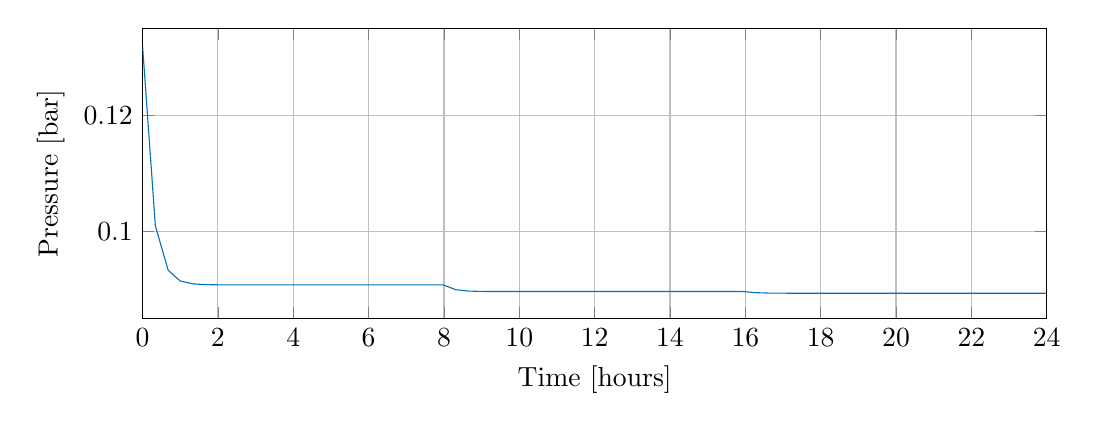
\begin{tikzpicture}

\begin{axis}[%
width=4.521in,
height=1.453in,
at={(1.011in,0.642in)},
scale only axis,
xmin=0,
xmax=24,
xlabel={Time [hours]},
xmajorgrids,
ymin=0.085,
ymax=0.135,
ylabel={Pressure [bar]},
ymajorgrids,
axis background/.style={fill=white}
]
\addplot [color=mycolor1,solid,forget plot]
  table[row sep=crcr]{%
0	0.132\\
0.340448888888889	0.10098922381935\\
0.680897777777778	0.0933420555374303\\
0.997028888888889	0.09152120078485\\
1.33747777777778	0.091007268267994\\
1.67792666666667	0.0908805339863671\\
1.99405777777778	0.0908503574935128\\
2.33450666666667	0.0908418402403378\\
2.67495555555556	0.0908397399101833\\
2.99108666666667	0.0908392398039998\\
3.33153555555556	0.0908390986500559\\
3.67198444444444	0.090839063841899\\
3.98811555555556	0.0908390555537856\\
4.32856444444444	0.0908390532144826\\
4.66901333333333	0.0908390526376172\\
4.98514444444444	0.0908390525002607\\
5.32559333333333	0.0908390524614921\\
5.64172444444444	0.090839052452261\\
5.98217333333333	0.0908390524496556\\
6.32262222222222	0.0908390524490131\\
6.63875333333333	0.0908390524488601\\
6.97920222222222	0.0908390524488169\\
7.31965111111111	0.0908390524488062\\
7.63578222222222	0.0908390524488037\\
7.97623111111111	0.090839052448803\\
8.31668	0.0900045989686734\\
8.63281111111111	0.0897771837267325\\
8.97326	0.0897129962414339\\
9.31370888888889	0.0896971677920325\\
9.62984	0.0896933989057918\\
9.97028888888889	0.0896923351453855\\
10.28642	0.0896920818551321\\
10.6268688888889	0.089692010364478\\
10.9673177777778	0.0896919927350881\\
11.2834488888889	0.0896919885373829\\
11.6238977777778	0.0896919873525892\\
11.9643466666667	0.0896919870604225\\
12.2804777777778	0.0896919869908551\\
12.6209266666667	0.0896919869712199\\
12.9613755555556	0.0896919869663779\\
13.2775066666667	0.089691986965225\\
13.6179555555556	0.0896919869648996\\
13.9340866666667	0.0896919869648221\\
14.2745355555556	0.0896919869648002\\
14.6149844444444	0.0896919869647948\\
14.9311155555556	0.0896919869647935\\
15.2715644444444	0.0896919869647932\\
15.5633777777778	0.0896919869647931\\
15.6120133333333	0.0896919869647931\\
15.9281444444444	0.0896919869647931\\
16.2685933333333	0.0894996962770216\\
16.6090422222222	0.0894274106144457\\
16.9251733333333	0.0894101987933647\\
17.2656222222222	0.0894053407921896\\
17.6060711111111	0.0894041428230615\\
17.9222022222222	0.0894038575765886\\
18.2626511111111	0.0894037770663571\\
18.6031	0.0894037572127653\\
18.9192311111111	0.089403752485459\\
19.25968	0.0894037511511866\\
19.5758111111111	0.0894037508334851\\
19.91626	0.0894037507438145\\
20.2567088888889	0.089403750721702\\
20.57284	0.0894037507164368\\
20.9132888888889	0.0894037507149508\\
21.2537377777778	0.0894037507145843\\
21.5698688888889	0.089403750714497\\
21.9103177777778	0.0894037507144724\\
22.2507666666667	0.0894037507144663\\
22.5668977777778	0.0894037507144649\\
22.9073466666667	0.0894037507144645\\
23.0532533333333	0.0894037507144644\\
23.2234777777778	0.0894037507144644\\
23.5639266666667	0.0894037507144644\\
23.9043755555556	0.0894037507144644\\
24.2205066666667	0.0893253001935264\\
24.5609555555556	0.0892848063842356\\
24.9014044444444	0.0892748207272428\\
25.2175355555556	0.0892724430587617\\
25.5579844444444	0.0892717719667128\\
25.8984333333333	0.0892716064773422\\
26.2145644444444	0.0892715670729384\\
26.5550133333333	0.0892715559511263\\
26.8954622222222	0.0892715532085194\\
27.2115933333333	0.0892715525554818\\
27.5520422222222	0.0892715523711632\\
27.8681733333333	0.0892715523272755\\
28.2086222222222	0.0892715523148882\\
28.5490711111111	0.0892715523118336\\
28.8652022222222	0.0892715523111062\\
29.2056511111111	0.0892715523109009\\
29.5461	0.0892715523108503\\
29.8622311111111	0.0892715523108382\\
30.20268	0.0892715523108348\\
30.5431288888889	0.089271552310834\\
30.85926	0.0892715523108338\\
30.9808488888889	0.0892715523108338\\
31.1997088888889	0.0892715523108338\\
31.5401577777778	0.0892715523108338\\
31.8562888888889	0.0892715523108338\\
32.1967377777778	0.0892715523108338\\
32.5128688888889	0.0892715523108338\\
32.8533177777778	0.0892715523108338\\
33.1937666666667	0.0892715523108338\\
33.5098977777778	0.0892715523108338\\
33.8503466666667	0.0892715523108338\\
34.1907955555556	0.0892715523108338\\
34.5069266666667	0.0892715523108338\\
34.8473755555556	0.0892715523108338\\
35.1878244444444	0.0892715523108338\\
35.5039555555555	0.0892715523108338\\
35.8444044444444	0.0892715523108338\\
36.1848533333333	0.0892715523108338\\
36.5009844444444	0.0892715523108338\\
36.8414333333333	0.0892715523108338\\
37.1818822222222	0.0892715523108338\\
37.4980133333333	0.0892715523108338\\
37.8384622222222	0.0892715523108338\\
38.1545933333333	0.0892715523108338\\
38.4950422222222	0.0892715523108338\\
38.8354911111111	0.0892715523108338\\
39.1516222222222	0.0892715523108338\\
39.4920711111111	0.0892715523108338\\
39.83252	0.0892715523108338\\
40.1486511111111	0.0892715523108338\\
40.4891	0.0892715523108338\\
40.8295488888889	0.0892715523108338\\
41.14568	0.0892715523108338\\
41.4861288888889	0.0892715523108338\\
41.8265777777778	0.0892715523108338\\
42.1427088888889	0.0892715523108338\\
42.4831577777778	0.0892715523108338\\
42.7992888888889	0.0892715523108338\\
43.1397377777778	0.0892715523108338\\
43.4801866666667	0.0892715523108338\\
43.7963177777778	0.0892715523108338\\
44.1367666666667	0.0892715523108338\\
44.4772155555556	0.0892715523108338\\
44.7933466666667	0.0892715523108338\\
45.1337955555556	0.0892715523108338\\
45.4742444444444	0.0892715523108338\\
45.7903755555555	0.0892715523108338\\
46.1308244444444	0.0892715523108338\\
46.4469555555556	0.0892715523108338\\
46.7874044444444	0.0892715523108338\\
47.1278533333333	0.0892715523108338\\
47.4439844444444	0.0892715523108338\\
47.7844333333333	0.0892715523108338\\
48.1248822222222	0.0892715523108338\\
48.4410133333333	0.0892715523108338\\
48.7814622222222	0.0892715523108338\\
49.1219111111111	0.089274623063706\\
49.4380422222222	0.0892780665701992\\
49.7784911111111	0.0892790384928396\\
50.11894	0.0892792781661694\\
50.4350711111111	0.0892793352343946\\
50.77552	0.0892793513417841\\
51.1159688888889	0.08927935531382\\
51.4321	0.089279356259595\\
51.7725488888889	0.0892793565265381\\
52.08868	0.0892793565900994\\
52.4291288888889	0.0892793566080395\\
52.7695777777778	0.0892793566124635\\
53.0857088888889	0.0892793566135169\\
53.4261577777778	0.0892793566138142\\
53.7666066666667	0.0892793566138875\\
54.0827377777778	0.0892793566139049\\
54.4231866666667	0.0892793566139099\\
54.7636355555556	0.0892793566139111\\
55.0554488888889	0.0892793566139114\\
55.0797666666667	0.0892793566139114\\
55.3229444444444	0.0892793566139115\\
55.4202155555556	0.0892793566139115\\
55.7363466666667	0.0892793566139115\\
56.0767955555556	0.0892793566139115\\
56.4172444444444	0.0892793566139115\\
56.7333755555556	0.0892793566139115\\
57.0738244444444	0.0893530006522183\\
57.4142733333333	0.0895115893716134\\
57.7304044444444	0.0895493506726297\\
58.0708533333333	0.0895600087223416\\
58.4113022222222	0.0895626369667696\\
58.7274333333333	0.0895632627737587\\
59.0678822222222	0.0895634394064969\\
59.4083311111111	0.0895634829636226\\
59.7244622222222	0.0895634933349386\\
60.0649111111111	0.0895634962622213\\
60.40536	0.0895634969840808\\
60.7214911111111	0.0895634971559616\\
61.06194	0.0895634972044746\\
61.3780711111111	0.0895634972160259\\
61.71852	0.0895634972192863\\
62.0589688888889	0.0895634972200903\\
62.3751	0.0895634972202817\\
62.7155488888889	0.0895634972203357\\
63.0559977777778	0.0895634972203491\\
63.3721288888889	0.0895634972203522\\
63.7125777777778	0.0895634972203531\\
64.0530266666667	0.0895634972203534\\
64.1746155555555	0.0895634972203534\\
64.3691577777778	0.0895634972203534\\
64.7096066666667	0.0895634972203534\\
65.0257377777778	0.0895543368455904\\
65.3661866666667	0.0894887155102987\\
65.7066355555556	0.08947253347761\\
66.0227666666667	0.08946868040023\\
66.3632155555556	0.0894675928770475\\
66.7036644444444	0.0894673246969562\\
67.0197955555556	0.0894672608410325\\
67.3602444444444	0.0894672428178291\\
67.7006933333333	0.089467238373359\\
68.0168244444444	0.0894672373150935\\
68.3572733333333	0.0894672370164002\\
68.6977222222222	0.0894672369427433\\
69.0138533333333	0.0894672369252049\\
69.3543022222222	0.0894672369202548\\
69.6704333333333	0.0894672369190761\\
70.0108822222222	0.0894672369187434\\
70.3513311111111	0.0894672369186614\\
70.6674622222222	0.0894672369186419\\
71.0079111111111	0.0894672369186364\\
71.34836	0.089467236918635\\
71.6644911111111	0.0894672369186347\\
71.8833511111111	0.0894672369186346\\
72.00494	0.0894672369186346\\
72.3453888888889	0.0894672369186346\\
72.66152	0.0894672369186346\\
73.0019688888889	0.0894672369186346\\
73.3424177777778	0.0894672369186346\\
73.6585488888889	0.0894672369186346\\
73.9989977777778	0.0894672369186346\\
74.3394466666667	0.0894672369186346\\
74.6555777777778	0.0894672369186346\\
74.9960266666667	0.0894672369186346\\
75.3121577777778	0.0894672369186346\\
75.6526066666667	0.0894672369186346\\
75.9930555555556	0.0894672369186346\\
76.3091866666667	0.0894672369186346\\
76.6496355555555	0.0894672369186346\\
76.9900844444444	0.0894672369186346\\
77.3062155555556	0.0894672369186346\\
77.6466644444444	0.0894672369186346\\
77.9871133333333	0.0894672369186346\\
78.3032444444444	0.0894672369186346\\
78.6436933333333	0.0894672369186346\\
78.9598244444445	0.0894672369186346\\
79.3002733333333	0.0894672369186346\\
79.6407222222222	0.0894672369186346\\
79.9568533333333	0.0894672369186346\\
80.2973022222222	0.0894672369186346\\
80.6377511111111	0.0894672369186346\\
80.9538822222222	0.0894672369186346\\
81.2943311111111	0.0894672369186346\\
81.63478	0.0894672369186346\\
81.9509111111111	0.0894672369186346\\
82.29136	0.0894672369186346\\
82.6318088888889	0.0894672369186346\\
82.94794	0.0894672369186346\\
83.2883888888889	0.0894672369186346\\
83.6288377777778	0.0894672369186346\\
83.9449688888889	0.0894672369186346\\
84.2854177777778	0.0894672369186346\\
84.6015488888889	0.0894672369186346\\
84.9419977777778	0.0894672369186346\\
85.2824466666667	0.0894672369186346\\
85.5985777777778	0.0894672369186346\\
85.9390266666667	0.0894672369186346\\
86.2794755555555	0.0894672369186346\\
86.5956066666667	0.0894672369186346\\
86.9360555555556	0.0894672369186346\\
87.2765044444444	0.0894672369186346\\
87.5926355555556	0.0894672369186346\\
87.9330844444444	0.0894672369186346\\
88.2735333333333	0.0894672369186346\\
88.5896644444445	0.0894672369186346\\
88.9301133333333	0.0894672369186346\\
89.2462444444444	0.0894672369186346\\
89.5866933333333	0.0894672369186346\\
89.9271422222222	0.0894672369186346\\
90.2432733333333	0.0894987065091299\\
90.5837222222222	0.0895125047680292\\
90.9241711111111	0.0895159073790179\\
91.2403022222222	0.0895167175691644\\
91.5807511111111	0.0895169462436704\\
91.9212	0.0895170026341464\\
92.2373311111111	0.0895170160611905\\
92.57778	0.0895170198509462\\
92.8939111111111	0.0895170207533187\\
93.23436	0.0895170210080115\\
93.5748088888889	0.089517021070818\\
93.89094	0.0895170210857728\\
94.2313888888889	0.0895170210899937\\
94.5718377777778	0.0895170210910346\\
94.8879688888889	0.0895170210912824\\
95.2284177777778	0.0895170210913524\\
95.5688666666667	0.0895170210913696\\
95.8849977777778	0.0895170210913737\\
96.2254466666667	0.0895170210913749\\
96.5658955555556	0.0895170210913752\\
96.7604377777778	0.0895170210913752\\
96.8820266666667	0.0895170210913752\\
97.2224755555556	0.0895170210913752\\
97.5386066666667	0.0895170210913752\\
97.8790555555556	0.0895170210913752\\
98.2195044444445	0.089308519529461\\
98.5356355555556	0.089204602012738\\
98.8760844444444	0.0891752715069196\\
99.2165333333333	0.08916803868848\\
99.5326644444444	0.0891663164938918\\
99.8731133333333	0.0891658304080038\\
100.213562222222	0.0891657105406209\\
100.529693333333	0.089165681999194\\
100.870142222222	0.0891656739434349\\
101.210591111111	0.0891656719569078\\
101.526722222222	0.0891656714838991\\
101.867171111111	0.0891656713503934\\
102.20762	0.0891656713174713\\
102.523751111111	0.0891656713096322\\
102.8642	0.0891656713074197\\
103.180331111111	0.0891656713068928\\
103.52078	0.0891656713067442\\
103.861228888889	0.0891656713067075\\
104.17736	0.0891656713066988\\
104.517808888889	0.0891656713066963\\
104.858257777778	0.0891656713066957\\
105.174388888889	0.0891656713066955\\
105.27166	0.0891656713066955\\
105.514837777778	0.0891656713066955\\
105.855286666667	0.0891656713066955\\
106.171417777778	0.08939861992079\\
106.511866666667	0.0895717432758513\\
106.852315555556	0.0896144349976571\\
107.168446666667	0.0896246002538251\\
107.508895555556	0.0896274693765157\\
107.825026666667	0.0896281525386346\\
108.165475555556	0.0896283453597406\\
108.505924444444	0.0896283929088711\\
108.822055555556	0.089628404230717\\
109.162504444444	0.0896284074262847\\
109.502953333333	0.0896284082143025\\
109.819084444444	0.0896284084019362\\
110.159533333333	0.0896284084548954\\
110.499982222222	0.089628408467955\\
110.816113333333	0.0896284084710646\\
111.156562222222	0.0896284084719422\\
111.472693333333	0.0896284084721512\\
111.813142222222	0.0896284084722102\\
112.153591111111	0.0896284084722248\\
112.469722222222	0.0896284084722282\\
112.810171111111	0.0896284084722292\\
113.15062	0.0896284084722294\\
113.320844444444	0.0896284084722295\\
113.466751111111	0.0896284084722295\\
113.8072	0.0896284084722295\\
114.147648888889	0.089605670533556\\
114.46378	0.0895855504073479\\
114.804228888889	0.0895798715430195\\
115.144677777778	0.0895784711513971\\
115.460808888889	0.0895781377064346\\
115.801257777778	0.0895780435922782\\
116.141706666667	0.0895780203839978\\
116.457837777778	0.089578014857912\\
116.798286666667	0.0895780132981856\\
117.114417777778	0.0895780129268017\\
117.454866666667	0.0895780128219794\\
117.795315555556	0.0895780127961305\\
118.111446666667	0.0895780127899757\\
118.451895555556	0.0895780127882385\\
118.792344444444	0.0895780127878101\\
119.108475555556	0.0895780127877081\\
119.448924444444	0.0895780127876793\\
119.789373333333	0.0895780127876722\\
120.105504444444	0.0895780127876705\\
120.445953333333	0.08957801278767\\
120.786402222222	0.0895780127876699\\
121.102533333333	0.0895780127876699\\
121.442982222222	0.0895780127876699\\
121.759113333333	0.0895780127876699\\
122.099562222222	0.0895780127876699\\
122.440011111111	0.0895780127876699\\
122.756142222222	0.0895780127876699\\
123.096591111111	0.0895780127876699\\
123.43704	0.0895780127876699\\
123.753171111111	0.0895780127876699\\
124.09362	0.0895780127876699\\
124.434068888889	0.0895780127876699\\
124.7502	0.0895780127876699\\
125.090648888889	0.0895780127876699\\
125.431097777778	0.0895780127876699\\
125.747228888889	0.0895780127876699\\
126.087677777778	0.0895780127876699\\
126.403808888889	0.0895780127876699\\
126.744257777778	0.0895780127876699\\
127.084706666667	0.0895780127876699\\
127.400837777778	0.0895780127876699\\
127.741286666667	0.0895780127876699\\
128.081735555556	0.0895780127876699\\
128.397866666667	0.0895780127876699\\
128.738315555556	0.0895780127876699\\
129.078764444444	0.0895780127876699\\
129.394895555556	0.0895780127876699\\
129.735344444444	0.0895780127876699\\
130.051475555556	0.0895780127876699\\
130.391924444444	0.0895780127876699\\
130.732373333333	0.0895780127876699\\
131.048504444444	0.0895780127876699\\
131.388953333333	0.0895780127876699\\
131.729402222222	0.0895780127876699\\
132.045533333333	0.0895780127876699\\
132.385982222222	0.0895780127876699\\
132.726431111111	0.0895780127876699\\
133.042562222222	0.0895780127876699\\
133.383011111111	0.0895780127876699\\
133.72346	0.0895780127876699\\
134.039591111111	0.0895780127876699\\
134.38004	0.0895780127876699\\
134.696171111111	0.0895780127876699\\
135.03662	0.0895780127876699\\
135.377068888889	0.0895780127876699\\
135.6932	0.0895780127876699\\
136.033648888889	0.0895780127876699\\
136.374097777778	0.0895780127876699\\
136.690228888889	0.0895780127876699\\
137.030677777778	0.0895780127876699\\
137.371126666667	0.0895780127876699\\
137.687257777778	0.0895780127876699\\
138.027706666667	0.0895780127876699\\
138.368155555556	0.0895780127876699\\
138.684286666667	0.0895780127876699\\
139.024735555556	0.0895893830770838\\
139.340866666667	0.0896680314942838\\
139.681315555556	0.0896902298486232\\
140.021764444444	0.0896957038990057\\
140.337895555556	0.0896970073162038\\
140.678344444444	0.0896973752030328\\
141.018793333333	0.0896974659228676\\
141.334924444444	0.0896974875240193\\
141.675373333333	0.0896974936209\\
142.015822222222	0.0896974951243733\\
142.331953333333	0.0896974954823629\\
142.672402222222	0.0896974955834047\\
143.012851111111	0.0896974956083213\\
143.328982222222	0.0896974956142541\\
143.669431111111	0.0896974956159287\\
143.985562222222	0.0896974956163274\\
};
\end{axis}
\end{tikzpicture}% 
\caption{WT pressure with all the constraints.}
\label{fig:Output_input}
\end{figure}

\begin{figure}[H]
\centering
% This file was created by matlab2tikz.
%
%The latest updates can be retrieved from
%  http://www.mathworks.com/matlabcentral/fileexchange/22022-matlab2tikz-matlab2tikz
%where you can also make suggestions and rate matlab2tikz.
%
\definecolor{mycolor1}{rgb}{0.00000,0.44700,0.74100}%
\definecolor{mycolor2}{rgb}{0.85000,0.32500,0.09800}%
%
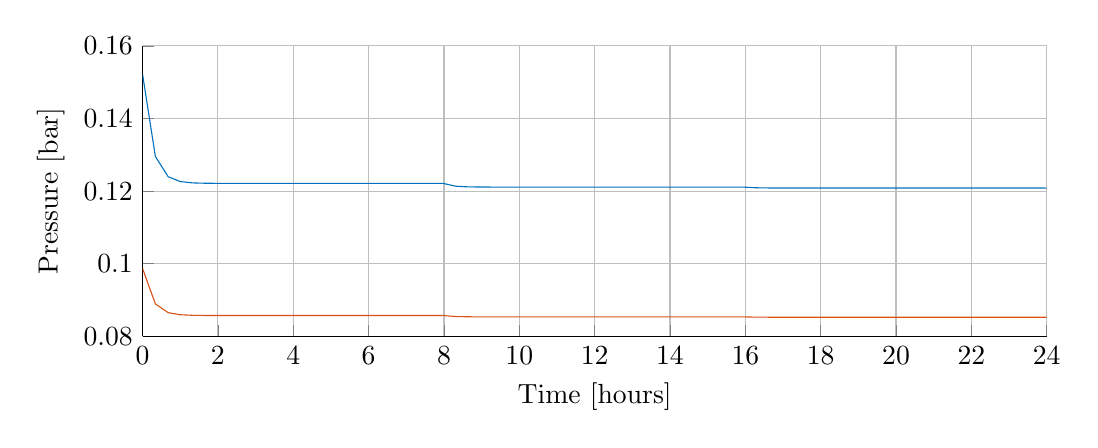
\begin{tikzpicture}

\begin{axis}[%
scaled y ticks = false,
 y tick label style={/pgf/number format/fixed,
/pgf/number format/1000 sep = \thinspace}, % Optional if you want to replace comma as the 1000 separator
width=4.521in,
height=1.453in,
at={(1.011in,0.642in)},
scale only axis,
xmin=0,
xmax=24,
xlabel={Time [hours]},
xmajorgrids,
ymin=0.08,
ymax=0.16,
ylabel={Pressure [bar]},
ymajorgrids,
axis background/.style={fill=white},
axis x line*=bottom,
axis y line*=left
]
\addplot [color=mycolor1,solid,forget plot]
  table[row sep=crcr]{%
0	0.15218792158004\\
0.340448888888889	0.129544081298018\\
0.680897777777778	0.123960175362327\\
0.997028888888889	0.122630600637915\\
1.33747777777778	0.122255330900723\\
1.67792666666667	0.122162790462048\\
1.99405777777778	0.122140755809303\\
2.33450666666667	0.12213453657379\\
2.67495555555556	0.122133002928186\\
2.99108666666667	0.122132637754335\\
3.33153555555556	0.122132534684766\\
3.67198444444444	0.122132509268106\\
3.98811555555556	0.122132503216187\\
4.32856444444444	0.122132501508045\\
4.66901333333333	0.122132501086822\\
4.98514444444444	0.122132500986525\\
5.32559333333333	0.122132500958217\\
5.64172444444444	0.122132500951476\\
5.98217333333333	0.122132500949574\\
6.32262222222222	0.122132500949104\\
6.63875333333333	0.122132500948993\\
6.97920222222222	0.122132500948961\\
7.31965111111111	0.122132500948953\\
7.63578222222222	0.122132500948952\\
7.97623111111111	0.122132500948951\\
8.31668	0.121337996260055\\
8.63281111111111	0.121171939325968\\
8.97326	0.121125070097132\\
9.31370888888889	0.121113512280002\\
9.62984	0.121110760267038\\
9.97028888888889	0.121109983517027\\
10.28642	0.12110979856635\\
10.6268688888889	0.121109746364401\\
10.9673177777778	0.121109733491551\\
11.2834488888889	0.121109730426417\\
11.6238977777778	0.12110972956129\\
11.9643466666667	0.121109729347952\\
12.2804777777778	0.121109729297154\\
12.6209266666667	0.121109729282816\\
12.9613755555556	0.121109729279281\\
13.2775066666667	0.121109729278439\\
13.6179555555556	0.121109729278201\\
13.9584044444444	0.121109729278143\\
14.2745355555556	0.121109729278129\\
14.6149844444444	0.121109729278125\\
14.9311155555556	0.121109729278124\\
15.2715644444444	0.121109729278124\\
15.53906	0.121109729278124\\
15.6120133333333	0.121109729278124\\
15.9281444444444	0.121109729278124\\
16.2685933333333	0.120922822836654\\
16.6090422222222	0.120870040378437\\
16.9251733333333	0.120857472433499\\
17.2656222222222	0.120853925156834\\
17.6060711111111	0.120853050408603\\
17.9222022222222	0.12085284212373\\
18.2626511111111	0.120852783335752\\
18.6031	0.120852768838806\\
18.9192311111111	0.120852765386962\\
19.25968	0.120852764412686\\
19.6001288888889	0.120852764172432\\
19.91626	0.120852764115226\\
20.2567088888889	0.120852764099079\\
20.57284	0.120852764095235\\
20.9132888888889	0.12085276409415\\
21.2537377777778	0.120852764093882\\
21.5698688888889	0.120852764093818\\
21.9103177777778	0.1208527640938\\
22.2507666666667	0.120852764093796\\
22.5668977777778	0.120852764093795\\
22.8830288888889	0.120852764093795\\
22.9073466666667	0.120852764093795\\
23.0532533333333	0.120852764093795\\
23.2477955555556	0.120852764093795\\
23.5639266666667	0.120852764093795\\
23.9043755555556	0.120852764093795\\
24.2448244444444	0.120770431554261\\
24.5609555555556	0.1207445980514\\
24.9014044444444	0.120737306598238\\
25.2175355555556	0.120735570442231\\
25.5579844444444	0.120735080415762\\
25.8984333333333	0.120734959576643\\
26.2145644444444	0.120734930803837\\
26.5550133333333	0.120734922682772\\
26.8954622222222	0.120734920680141\\
27.2115933333333	0.120734920203297\\
27.5520422222222	0.120734920068709\\
27.8924911111111	0.12073492003552\\
28.2086222222222	0.120734920027618\\
28.5490711111111	0.120734920025387\\
28.88952	0.120734920024837\\
29.2056511111111	0.120734920024706\\
29.5461	0.120734920024669\\
29.8622311111111	0.120734920024661\\
30.20268	0.120734920024658\\
30.5431288888889	0.120734920024657\\
30.85926	0.120734920024657\\
31.0294844444444	0.120734920024657\\
31.1997088888889	0.120734920024657\\
31.5401577777778	0.120734920024657\\
31.8562888888889	0.120734920024657\\
32.1967377777778	0.120734920024657\\
32.5371866666667	0.120734920024657\\
32.8533177777778	0.120734920024657\\
33.1937666666667	0.120734920024657\\
33.5342155555556	0.120734920024657\\
33.8503466666667	0.120734920024657\\
34.1907955555556	0.120734920024657\\
34.5069266666667	0.120734920024657\\
34.8473755555556	0.120734920024657\\
35.1878244444444	0.120734920024657\\
35.5039555555555	0.120734920024657\\
35.8444044444444	0.120734920024657\\
36.1848533333333	0.120734920024657\\
36.5009844444444	0.120734920024657\\
36.8414333333333	0.120734920024657\\
37.1818822222222	0.120734920024657\\
37.4980133333333	0.120734920024657\\
37.8384622222222	0.120734920024657\\
38.1789111111111	0.120734920024657\\
38.4950422222222	0.120734920024657\\
38.8354911111111	0.120734920024657\\
39.17594	0.120734920024657\\
39.4920711111111	0.120734920024657\\
39.83252	0.120734920024657\\
40.1486511111111	0.120734920024657\\
40.4891	0.120734920024657\\
40.8295488888889	0.120734920024657\\
41.14568	0.120734920024657\\
41.4861288888889	0.120734920024657\\
41.8265777777778	0.120734920024657\\
42.1427088888889	0.120734920024657\\
42.4831577777778	0.120734920024657\\
42.8236066666667	0.120734920024657\\
43.1397377777778	0.120734920024657\\
43.4801866666667	0.120734920024657\\
43.8206355555556	0.120734920024657\\
44.1367666666667	0.120734920024657\\
44.4772155555556	0.120734920024657\\
44.7933466666667	0.120734920024657\\
45.1337955555556	0.120734920024657\\
45.4742444444444	0.120734920024657\\
45.7903755555555	0.120734920024657\\
46.1308244444444	0.120734920024657\\
46.4712733333333	0.120734920024657\\
46.7874044444444	0.120734920024657\\
47.1278533333333	0.120734920024657\\
47.4683022222222	0.120734920024657\\
47.7844333333333	0.120734920024657\\
48.1248822222222	0.120734920024657\\
48.4653311111111	0.120734920024657\\
48.7814622222222	0.120734920024657\\
49.1219111111111	0.120738417932083\\
49.4380422222222	0.120740932355153\\
49.7784911111111	0.120741642045904\\
50.11894	0.120741817053603\\
50.4350711111111	0.120741858724401\\
50.77552	0.120741870485898\\
51.1159688888889	0.120741873386249\\
51.4321	0.120741874076847\\
51.7725488888889	0.120741874271767\\
52.1129977777778	0.120741874319834\\
52.4291288888889	0.120741874331279\\
52.7695777777778	0.120741874334509\\
53.1100266666667	0.120741874335306\\
53.4261577777778	0.120741874335495\\
53.7666066666667	0.120741874335549\\
54.1070555555556	0.120741874335562\\
54.4231866666667	0.120741874335565\\
54.7636355555556	0.120741874335566\\
55.0554488888889	0.120741874335566\\
55.0797666666667	0.120741874335566\\
55.2986266666667	0.120741874335566\\
55.4202155555556	0.120741874335566\\
55.7606644444444	0.120741874335566\\
56.0767955555556	0.120741874335566\\
56.4172444444444	0.120741874335566\\
56.7576933333333	0.120741874335566\\
57.0738244444444	0.120841485565655\\
57.4142733333333	0.120957285880087\\
57.7547222222222	0.120985841904819\\
58.0708533333333	0.120992641333239\\
58.4113022222222	0.120994560457955\\
58.7517511111111	0.120995033708595\\
59.0678822222222	0.120995146393532\\
59.4083311111111	0.120995178198624\\
59.7244622222222	0.120995185771683\\
60.0649111111111	0.120995187909163\\
60.40536	0.120995188436259\\
60.7214911111111	0.120995188561766\\
61.06194	0.120995188597189\\
61.4023888888889	0.120995188605925\\
61.71852	0.120995188608005\\
62.0589688888889	0.120995188608592\\
62.3994177777778	0.120995188608737\\
62.7155488888889	0.120995188608771\\
63.0559977777778	0.120995188608781\\
63.3964466666667	0.120995188608783\\
63.7125777777778	0.120995188608784\\
64.0043911111111	0.120995188608784\\
64.0530266666667	0.120995188608784\\
64.1502977777778	0.120995188608784\\
64.3691577777778	0.120995188608784\\
64.7096066666667	0.120995188608784\\
65.0500555555555	0.120966840502907\\
65.3661866666667	0.120924976598704\\
65.7066355555556	0.120913160597662\\
66.0470844444444	0.120910246805764\\
66.3632155555556	0.120909553007534\\
66.7036644444444	0.120909357184407\\
67.0441133333333	0.120909308894986\\
67.3602444444444	0.120909297396871\\
67.7006933333333	0.120909294151552\\
68.0411422222222	0.120909293351266\\
68.3572733333333	0.120909293160711\\
68.6977222222222	0.120909293106927\\
69.0138533333333	0.120909293094121\\
69.3543022222222	0.120909293090506\\
69.6947511111111	0.120909293089615\\
70.0108822222222	0.120909293089403\\
70.3513311111111	0.120909293089343\\
70.69178	0.120909293089328\\
71.0079111111111	0.120909293089324\\
71.34836	0.120909293089323\\
71.6888088888889	0.120909293089323\\
71.9319866666667	0.120909293089323\\
72	0.120909293089323\\
72.3453888888889	0.120909293089323\\
72.6858377777778	0.120909293089323\\
73	0.120909293089323\\
73.3424177777778	0.120909293089323\\
73.6828666666667	0.120909293089323\\
73.9989977777778	0.120909293089323\\
74.3394466666667	0.120909293089323\\
74.6555777777778	0.120909293089323\\
74.9960266666667	0.120909293089323\\
75.3364755555556	0.120909293089323\\
75.6526066666667	0.120909293089323\\
75.9930555555556	0.120909293089323\\
76.3335044444444	0.120909293089323\\
76.6496355555555	0.120909293089323\\
76.9900844444444	0.120909293089323\\
77.3305333333333	0.120909293089323\\
77.6466644444444	0.120909293089323\\
77.9871133333333	0.120909293089323\\
78.3275622222222	0.120909293089323\\
78.6436933333333	0.120909293089323\\
78.9841422222222	0.120909293089323\\
79.3002733333333	0.120909293089323\\
79.6407222222222	0.120909293089323\\
79.9811711111111	0.120909293089323\\
80.2973022222222	0.120909293089323\\
80.6377511111111	0.120909293089323\\
80.9782	0.120909293089323\\
81.2943311111111	0.120909293089323\\
81.63478	0.120909293089323\\
81.9752288888889	0.120909293089323\\
82.29136	0.120909293089323\\
82.6318088888889	0.120909293089323\\
82.9722577777778	0.120909293089323\\
83.2883888888889	0.120909293089323\\
83.6288377777778	0.120909293089323\\
83.9449688888889	0.120909293089323\\
84.2854177777778	0.120909293089323\\
84.6258666666667	0.120909293089323\\
84.9419977777778	0.120909293089323\\
85.2824466666667	0.120909293089323\\
85.6228955555556	0.120909293089323\\
85.9390266666667	0.120909293089323\\
86.2794755555555	0.120909293089323\\
86.6199244444445	0.120909293089323\\
86.9360555555556	0.120909293089323\\
87.2765044444444	0.120909293089323\\
87.6169533333333	0.120909293089323\\
87.9330844444444	0.120909293089323\\
88.2735333333333	0.120909293089323\\
88.6139822222222	0.120909293089323\\
88.9301133333333	0.120909293089323\\
89.2705622222222	0.120909293089323\\
89.5866933333333	0.120909293089323\\
89.9271422222222	0.120909293089323\\
90.2675911111111	0.120941641449338\\
90.5837222222222	0.120950444211217\\
90.9241711111111	0.120952928772691\\
91.26462	0.12095354145841\\
91.5807511111111	0.120953687344006\\
91.9212	0.120953728519916\\
92.2616488888889	0.120953738673777\\
92.57778	0.120953741091496\\
92.9182288888889	0.120953741773893\\
93.2586777777778	0.12095374194217\\
93.5748088888889	0.120953741982238\\
93.9152577777778	0.120953741993547\\
94.2313888888889	0.12095374199624\\
94.5718377777778	0.120953741997\\
94.9122866666667	0.120953741997187\\
95.2284177777778	0.120953741997232\\
95.5688666666667	0.120953741997244\\
95.9093155555556	0.120953741997248\\
96.2254466666667	0.120953741997248\\
96.5658955555556	0.120953741997248\\
96.73612	0.120953741997249\\
96.9063444444444	0.120953741997249\\
97.2224755555556	0.120953741997249\\
97.5629244444444	0.120953741997249\\
97.9033733333333	0.120953741997249\\
98.2195044444445	0.120744837422735\\
98.5599533333333	0.120666252440286\\
98.8760844444444	0.120647540698437\\
99.2165333333333	0.120642259347703\\
99.5569822222222	0.12064095698179\\
99.8731133333333	0.120640646877569\\
100.213562222222	0.12064055935129\\
100.554011111111	0.120640537767561\\
100.870142222222	0.120640532628294\\
101.210591111111	0.120640531177747\\
101.55104	0.120640530820046\\
101.867171111111	0.120640530734874\\
102.20762	0.120640530710835\\
102.548068888889	0.120640530704907\\
102.8642	0.120640530703495\\
103.204648888889	0.120640530703097\\
103.52078	0.120640530703002\\
103.861228888889	0.120640530702975\\
104.201677777778	0.120640530702969\\
104.517808888889	0.120640530702967\\
104.858257777778	0.120640530702967\\
105.198706666667	0.120640530702966\\
105.247342222222	0.120640530702966\\
105.514837777778	0.120640530702966\\
105.855286666667	0.120640530702966\\
106.195735555556	0.120901243676319\\
106.511866666667	0.121011689760956\\
106.852315555556	0.121042862941669\\
107.192764444444	0.121050550158442\\
107.508895555556	0.121052380549076\\
107.849344444444	0.121052897173075\\
108.189793333333	0.121053024571069\\
108.505924444444	0.121053054905597\\
108.846373333333	0.121053063467455\\
109.162504444444	0.121053065506105\\
109.502953333333	0.12105306608151\\
109.843402222222	0.121053066223403\\
110.159533333333	0.121053066257189\\
110.499982222222	0.121053066266725\\
110.840431111111	0.121053066269077\\
111.156562222222	0.121053066269637\\
111.497011111111	0.121053066269795\\
111.83746	0.121053066269834\\
112.153591111111	0.121053066269843\\
112.49404	0.121053066269846\\
112.834488888889	0.121053066269846\\
113.126302222222	0.121053066269847\\
113.15062	0.121053066269847\\
113.272208888889	0.121053066269847\\
113.491068888889	0.121053066269847\\
113.8072	0.121053066269847\\
114.147648888889	0.121028326525222\\
114.488097777778	0.121013111190841\\
114.804228888889	0.121009488292417\\
115.144677777778	0.121008465736772\\
115.485126666667	0.121008213577489\\
115.801257777778	0.121008153536254\\
116.141706666667	0.121008136589739\\
116.482155555556	0.121008132410777\\
116.798286666667	0.121008131415731\\
117.138735555556	0.121008131134881\\
117.479184444444	0.121008131065624\\
117.795315555556	0.121008131049134\\
118.135764444444	0.121008131044479\\
118.451895555556	0.121008131043371\\
118.792344444444	0.121008131043058\\
119.132793333333	0.121008131042981\\
119.448924444444	0.121008131042963\\
119.789373333333	0.121008131042958\\
120.129822222222	0.121008131042956\\
120.421635555556	0.121008131042956\\
120.445953333333	0.121008131042956\\
120.762084444444	0.121008131042956\\
120.786402222222	0.121008131042956\\
121.126851111111	0.121008131042956\\
121.442982222222	0.121008131042956\\
121.783431111111	0.121008131042956\\
122.12388	0.121008131042956\\
122.440011111111	0.121008131042956\\
122.78046	0.121008131042956\\
123.120908888889	0.121008131042956\\
123.43704	0.121008131042956\\
123.777488888889	0.121008131042956\\
124.09362	0.121008131042956\\
124.434068888889	0.121008131042956\\
124.774517777778	0.121008131042956\\
125.090648888889	0.121008131042956\\
125.431097777778	0.121008131042956\\
125.771546666667	0.121008131042956\\
126.087677777778	0.121008131042956\\
126.428126666667	0.121008131042956\\
126.768575555556	0.121008131042956\\
127.084706666667	0.121008131042956\\
127.425155555556	0.121008131042956\\
127.765604444444	0.121008131042956\\
128.081735555556	0.121008131042956\\
128.422184444444	0.121008131042956\\
128.738315555556	0.121008131042956\\
129.078764444444	0.121008131042956\\
129.419213333333	0.121008131042956\\
129.735344444444	0.121008131042956\\
130.075793333333	0.121008131042956\\
130.416242222222	0.121008131042956\\
130.732373333333	0.121008131042956\\
131.072822222222	0.121008131042956\\
131.413271111111	0.121008131042956\\
131.729402222222	0.121008131042956\\
132.069851111111	0.121008131042956\\
132.4103	0.121008131042956\\
132.726431111111	0.121008131042956\\
133.06688	0.121008131042956\\
133.383011111111	0.121008131042956\\
133.72346	0.121008131042956\\
134.063908888889	0.121008131042956\\
134.38004	0.121008131042956\\
134.720488888889	0.121008131042956\\
135.060937777778	0.121008131042956\\
135.377068888889	0.121008131042956\\
135.717517777778	0.121008131042956\\
136.057966666667	0.121008131042956\\
136.374097777778	0.121008131042956\\
136.714546666667	0.121008131042956\\
137.054995555556	0.121008131042956\\
137.371126666667	0.121008131042956\\
137.711575555556	0.121008131042956\\
138.027706666667	0.121008131042956\\
138.368155555556	0.121008131042956\\
138.708604444444	0.121008131042956\\
139.024735555556	0.121035681301076\\
139.365184444444	0.121095157168862\\
139.705633333333	0.121109823746925\\
140.021764444444	0.121113315981879\\
140.362213333333	0.121114301658028\\
140.702662222222	0.121114544722933\\
141.018793333333	0.121114602598721\\
141.359242222222	0.121114618934043\\
141.699691111111	0.121114622962286\\
142.015822222222	0.121114623921445\\
142.356271111111	0.121114624192165\\
142.69672	0.121114624258924\\
143.012851111111	0.12111462427482\\
143.3533	0.121114624279307\\
143.669431111111	0.121114624280375\\
144	0.121114624280666\\
};
\addplot [color=mycolor2,solid,forget plot]
  table[row sep=crcr]{%
0	0.0987188547264836\\
0.340448888888889	0.0889476753653489\\
0.680897777777778	0.0865381306170287\\
0.997028888888889	0.0859643978515412\\
1.33747777777778	0.0858024629559918\\
1.67792666666667	0.0857625302761463\\
1.99405777777778	0.0857530219709542\\
2.33450666666667	0.0857503382713283\\
2.67495555555556	0.0857496764787134\\
2.99108666666667	0.0857495189003545\\
3.33153555555556	0.0857494744241861\\
3.67198444444444	0.0857494634564908\\
3.98811555555556	0.0857494608449908\\
4.32856444444444	0.0857494601079003\\
4.66901333333333	0.0857494599261359\\
4.98514444444444	0.0857494598828563\\
5.32559333333333	0.0857494598706407\\
5.64172444444444	0.0857494598677321\\
5.98217333333333	0.0857494598669111\\
6.32262222222222	0.0857494598667086\\
6.63875333333333	0.0857494598666604\\
6.97920222222222	0.0857494598666468\\
7.31965111111111	0.0857494598666435\\
7.63578222222222	0.0857494598666427\\
7.97623111111111	0.0857494598666425\\
8.31668	0.0854733417184805\\
8.63281111111111	0.0854016854946725\\
8.97326	0.0853814606725675\\
9.31370888888889	0.085376473289562\\
9.62984	0.0853752857519385\\
9.97028888888889	0.0853749505718815\\
10.28642	0.0853748707627054\\
10.6268688888889	0.0853748482367293\\
10.9673177777778	0.0853748426818883\\
11.2834488888889	0.0853748413592342\\
11.6238977777778	0.0853748409859178\\
11.9643466666667	0.085374840893859\\
12.2804777777778	0.0853748408719391\\
12.6209266666667	0.0853748408657522\\
12.9613755555556	0.0853748408642266\\
13.2775066666667	0.0853748408638633\\
13.6179555555556	0.0853748408637608\\
13.9584044444444	0.0853748408637355\\
14.2745355555556	0.0853748408637295\\
14.6149844444444	0.0853748408637277\\
14.9311155555556	0.0853748408637273\\
15.2229288888889	0.0853748408637272\\
15.2715644444444	0.0853748408637272\\
15.4417888888889	0.0853748408637272\\
15.6120133333333	0.0853748408637272\\
15.9281444444444	0.0853748408637272\\
16.2685933333333	0.0853109041972383\\
16.6090422222222	0.0852881277220494\\
16.9251733333333	0.0852827044527338\\
17.2656222222222	0.0852811737461\\
17.6060711111111	0.0852807962782433\\
17.9222022222222	0.0852807063999883\\
18.2626511111111	0.0852806810320353\\
18.6031	0.085280674776371\\
18.9192311111111	0.085280673286845\\
19.25968	0.0852806728664293\\
19.6001288888889	0.0852806727627561\\
19.91626	0.0852806727380706\\
20.2567088888889	0.0852806727311032\\
20.57284	0.0852806727294441\\
20.9132888888889	0.0852806727289759\\
21.2537377777778	0.0852806727288604\\
21.5698688888889	0.0852806727288329\\
21.9103177777778	0.0852806727288252\\
22.2507666666667	0.0852806727288233\\
22.5668977777778	0.0852806727288228\\
22.8587111111111	0.0852806727288227\\
22.9073466666667	0.0852806727288227\\
23.0046177777778	0.0852806727288227\\
23.2477955555556	0.0852806727288227\\
23.5639266666667	0.0852806727288227\\
23.9043755555556	0.0852806727288227\\
24.2448244444444	0.0852527962619159\\
24.5609555555556	0.0852416486921206\\
24.9014044444444	0.0852385023134248\\
25.2175355555556	0.0852377531343312\\
25.5579844444444	0.0852375416800697\\
25.8984333333333	0.0852374895360565\\
26.2145644444444	0.0852374771201306\\
26.5550133333333	0.0852374736157611\\
26.8954622222222	0.0852374727515936\\
27.2115933333333	0.0852374725458281\\
27.5520422222222	0.0852374724877512\\
27.8924911111111	0.0852374724734296\\
28.2086222222222	0.0852374724700195\\
28.5490711111111	0.085237472469057\\
28.88952	0.0852374724688197\\
29.2056511111111	0.0852374724687631\\
29.5461	0.0852374724687472\\
29.8622311111111	0.0852374724687434\\
30.20268	0.0852374724687423\\
30.5431288888889	0.0852374724687421\\
30.7619888888889	0.085237472468742\\
30.85926	0.085237472468742\\
30.8835777777778	0.085237472468742\\
31.1997088888889	0.085237472468742\\
31.5401577777778	0.085237472468742\\
31.8562888888889	0.085237472468742\\
32.1967377777778	0.085237472468742\\
32.5371866666667	0.085237472468742\\
32.8533177777778	0.085237472468742\\
33.1937666666667	0.085237472468742\\
33.5342155555556	0.085237472468742\\
33.8503466666667	0.085237472468742\\
34.1907955555556	0.085237472468742\\
34.5069266666667	0.085237472468742\\
34.8473755555556	0.085237472468742\\
35.1878244444444	0.085237472468742\\
35.5039555555555	0.085237472468742\\
35.8444044444444	0.085237472468742\\
36.1848533333333	0.085237472468742\\
36.5009844444444	0.085237472468742\\
36.8414333333333	0.085237472468742\\
37.1818822222222	0.085237472468742\\
37.4980133333333	0.085237472468742\\
37.8384622222222	0.085237472468742\\
38.1789111111111	0.085237472468742\\
38.4950422222222	0.085237472468742\\
38.8354911111111	0.085237472468742\\
39.17594	0.085237472468742\\
39.4920711111111	0.085237472468742\\
39.83252	0.085237472468742\\
40.1486511111111	0.085237472468742\\
40.4891	0.085237472468742\\
40.8295488888889	0.085237472468742\\
41.14568	0.085237472468742\\
41.4861288888889	0.085237472468742\\
41.8265777777778	0.085237472468742\\
42.1427088888889	0.085237472468742\\
42.4831577777778	0.085237472468742\\
42.8236066666667	0.085237472468742\\
43.1397377777778	0.085237472468742\\
43.4801866666667	0.085237472468742\\
43.8206355555556	0.085237472468742\\
44.1367666666667	0.085237472468742\\
44.4772155555556	0.085237472468742\\
44.7933466666667	0.085237472468742\\
45.1337955555556	0.085237472468742\\
45.4742444444444	0.085237472468742\\
45.7903755555555	0.085237472468742\\
46.1308244444444	0.085237472468742\\
46.4712733333333	0.085237472468742\\
46.7874044444444	0.085237472468742\\
47.1278533333333	0.085237472468742\\
47.4683022222222	0.085237472468742\\
47.7844333333333	0.085237472468742\\
48.1248822222222	0.085237472468742\\
48.4653311111111	0.085237472468742\\
48.7814622222222	0.085237472468742\\
49.1219111111111	0.0852385335427205\\
49.4380422222222	0.0852396185565035\\
49.7784911111111	0.0852399247994169\\
50.11894	0.0852400003180392\\
50.4350711111111	0.085240018299655\\
50.77552	0.0852400233749292\\
51.1159688888889	0.0852400246264772\\
51.4321	0.0852400249244813\\
51.7725488888889	0.0852400250085923\\
52.1129977777778	0.0852400250293338\\
52.4291288888889	0.0852400250342726\\
52.7695777777778	0.0852400250356665\\
53.1100266666667	0.0852400250360103\\
53.4261577777778	0.0852400250360921\\
53.7666066666667	0.0852400250361152\\
54.1070555555556	0.0852400250361209\\
54.4231866666667	0.0852400250361223\\
54.7636355555556	0.0852400250361227\\
55.0311311111111	0.0852400250361227\\
55.0797666666667	0.0852400250361227\\
55.2743088888889	0.0852400250361228\\
55.4202155555556	0.0852400250361228\\
55.7606644444444	0.0852400250361228\\
56.0767955555556	0.0852400250361228\\
56.4172444444444	0.0852400250361228\\
56.7576933333333	0.0852400250361228\\
57.0738244444444	0.0852665294419842\\
57.4142733333333	0.0853164991303544\\
57.7547222222222	0.0853288215118947\\
58.0708533333333	0.0853317555740422\\
58.4113022222222	0.0853325837070615\\
58.7517511111111	0.085332787922284\\
59.0678822222222	0.0853328365476372\\
59.4083311111111	0.0853328502720433\\
59.7244622222222	0.0853328535399393\\
60.0649111111111	0.0853328544622962\\
60.40536	0.0853328546897468\\
60.7214911111111	0.0853328547439046\\
61.06194	0.0853328547591906\\
61.4023888888889	0.0853328547629601\\
61.71852	0.0853328547638576\\
62.0589688888889	0.0853328547641109\\
62.3994177777778	0.0853328547641734\\
62.7155488888889	0.0853328547641883\\
63.0559977777778	0.0853328547641925\\
63.3964466666667	0.0853328547641935\\
63.7125777777778	0.0853328547641938\\
64.0043911111111	0.0853328547641938\\
64.0530266666667	0.0853328547641938\\
64.1746155555555	0.0853328547641938\\
64.3691577777778	0.0853328547641938\\
64.7096066666667	0.0853328547641938\\
65.0500555555555	0.0853263070505115\\
65.3661866666667	0.085308242106066\\
65.7066355555556	0.0853031433125722\\
66.0470844444444	0.0853018859647504\\
66.3632155555556	0.0853015865797137\\
66.7036644444444	0.0853015020789015\\
67.0441133333333	0.0853014812412441\\
67.3602444444444	0.0853014762796235\\
67.7006933333333	0.0853014748792163\\
68.0411422222222	0.0853014745338799\\
68.3572733333333	0.0853014744516524\\
68.6977222222222	0.0853014744284438\\
69.0138533333333	0.0853014744229177\\
69.3543022222222	0.085301474421358\\
69.6947511111111	0.0853014744209733\\
70.0108822222222	0.0853014744208817\\
70.3513311111111	0.0853014744208559\\
70.69178	0.0853014744208495\\
71.0079111111111	0.085301474420848\\
71.34836	0.0853014744208476\\
71.6401733333333	0.0853014744208475\\
71.6888088888889	0.0853014744208475\\
71.8590333333333	0.0853014744208474\\
72	0.0853014744208474\\
72.3453888888889	0.0853014744208474\\
72.6858377777778	0.0853014744208474\\
73	0.0853014744208474\\
73.3424177777778	0.0853014744208474\\
73.6828666666667	0.0853014744208474\\
73.9989977777778	0.0853014744208474\\
74.3394466666667	0.0853014744208474\\
74.6555777777778	0.0853014744208474\\
74.9960266666667	0.0853014744208474\\
75.3364755555556	0.0853014744208474\\
75.6526066666667	0.0853014744208474\\
75.9930555555556	0.0853014744208474\\
76.3335044444444	0.0853014744208474\\
76.6496355555555	0.0853014744208474\\
76.9900844444444	0.0853014744208474\\
77.3305333333333	0.0853014744208474\\
77.6466644444444	0.0853014744208474\\
77.9871133333333	0.0853014744208474\\
78.3275622222222	0.0853014744208474\\
78.6436933333333	0.0853014744208474\\
78.9841422222222	0.0853014744208474\\
79.3002733333333	0.0853014744208474\\
79.6407222222222	0.0853014744208474\\
79.9811711111111	0.0853014744208474\\
80.2973022222222	0.0853014744208474\\
80.6377511111111	0.0853014744208474\\
80.9782	0.0853014744208474\\
81.2943311111111	0.0853014744208474\\
81.63478	0.0853014744208474\\
81.9752288888889	0.0853014744208474\\
82.29136	0.0853014744208474\\
82.6318088888889	0.0853014744208474\\
82.9722577777778	0.0853014744208474\\
83.2883888888889	0.0853014744208474\\
83.6288377777778	0.0853014744208474\\
83.9449688888889	0.0853014744208474\\
84.2854177777778	0.0853014744208474\\
84.6258666666667	0.0853014744208474\\
84.9419977777778	0.0853014744208474\\
85.2824466666667	0.0853014744208474\\
85.6228955555556	0.0853014744208474\\
85.9390266666667	0.0853014744208474\\
86.2794755555555	0.0853014744208474\\
86.6199244444445	0.0853014744208474\\
86.9360555555556	0.0853014744208474\\
87.2765044444444	0.0853014744208474\\
87.6169533333333	0.0853014744208474\\
87.9330844444444	0.0853014744208474\\
88.2735333333333	0.0853014744208474\\
88.6139822222222	0.0853014744208474\\
88.9301133333333	0.0853014744208474\\
89.2705622222222	0.0853014744208474\\
89.5866933333333	0.0853014744208474\\
89.9271422222222	0.0853014744208474\\
90.2675911111111	0.0853124602829105\\
90.5837222222222	0.0853162588154967\\
90.9241711111111	0.0853173309435232\\
91.26462	0.0853175953272133\\
91.5807511111111	0.085317658279182\\
91.9212	0.085317676047246\\
92.2616488888889	0.0853176804287995\\
92.57778	0.0853176814720841\\
92.9182288888889	0.085317681766549\\
93.2586777777778	0.0853176818391632\\
93.5748088888889	0.0853176818564533\\
93.9152577777778	0.0853176818613333\\
94.2313888888889	0.0853176818624953\\
94.5718377777778	0.0853176818628233\\
94.9122866666667	0.0853176818629042\\
95.2284177777778	0.0853176818629234\\
95.5688666666667	0.0853176818629289\\
95.9093155555556	0.0853176818629302\\
96.2254466666667	0.0853176818629305\\
96.5415777777778	0.0853176818629306\\
96.5658955555556	0.0853176818629306\\
96.7118022222222	0.0853176818629306\\
96.9063444444444	0.0853176818629306\\
97.2224755555556	0.0853176818629306\\
97.5629244444444	0.0853176818629306\\
97.9033733333333	0.0853176818629306\\
98.2195044444445	0.0852478867217642\\
98.5599533333333	0.0852139760445543\\
98.8760844444444	0.0852059016285764\\
99.2165333333333	0.0852036226412383\\
99.5569822222222	0.0852030606495105\\
99.8731133333333	0.0852029268345779\\
100.213562222222	0.0852028890655878\\
100.554011111111	0.0852028797518634\\
100.870142222222	0.0852028775341877\\
101.210591111111	0.0852028769082533\\
101.55104	0.0852028767538996\\
101.867171111111	0.0852028767171467\\
102.20762	0.0852028767067733\\
102.548068888889	0.0852028767042153\\
102.8642	0.0852028767036062\\
103.204648888889	0.0852028767034342\\
103.52078	0.0852028767033933\\
103.861228888889	0.0852028767033818\\
104.201677777778	0.0852028767033789\\
104.517808888889	0.0852028767033782\\
104.83394	0.085202876703378\\
104.858257777778	0.085202876703378\\
105.077117777778	0.085202876703378\\
105.198706666667	0.085202876703378\\
105.223024444444	0.085202876703378\\
105.514837777778	0.085202876703378\\
105.855286666667	0.085202876703378\\
106.195735555556	0.0852885401298615\\
106.511866666667	0.0853361993824125\\
106.852315555556	0.0853496511086308\\
107.192764444444	0.0853529682656563\\
107.508895555556	0.0853537581084991\\
107.849344444444	0.0853539810400204\\
108.189793333333	0.0853540360142929\\
108.505924444444	0.0853540491041271\\
108.846373333333	0.085354052798706\\
109.162504444444	0.0853540536784161\\
109.502953333333	0.0853540539267125\\
109.843402222222	0.0853540539879417\\
110.159533333333	0.0853540540025209\\
110.499982222222	0.0853540540066358\\
110.840431111111	0.0853540540076505\\
111.156562222222	0.0853540540078921\\
111.497011111111	0.0853540540079603\\
111.83746	0.0853540540079772\\
112.153591111111	0.0853540540079812\\
112.49404	0.0853540540079823\\
112.834488888889	0.0853540540079826\\
113.15062	0.0853540540079826\\
113.272208888889	0.0853540540079827\\
113.491068888889	0.0853540540079827\\
113.8072	0.0853540540079827\\
114.147648888889	0.0853463102839272\\
114.488097777778	0.0853397446237115\\
114.804228888889	0.0853381812850786\\
115.144677777778	0.085337740035958\\
115.485126666667	0.085337631225193\\
115.801257777778	0.0853376053164394\\
116.141706666667	0.0853375980037469\\
116.482155555556	0.0853375962004579\\
116.798286666667	0.0853375957710797\\
117.138735555556	0.0853375956498886\\
117.479184444444	0.0853375956200032\\
117.795315555556	0.0853375956128873\\
118.135764444444	0.0853375956108788\\
118.451895555556	0.0853375956104006\\
118.792344444444	0.0853375956102656\\
119.132793333333	0.0853375956102323\\
119.448924444444	0.0853375956102244\\
119.789373333333	0.0853375956102221\\
120.129822222222	0.0853375956102216\\
120.421635555556	0.0853375956102215\\
120.445953333333	0.0853375956102215\\
120.737766666667	0.0853375956102214\\
120.786402222222	0.0853375956102214\\
121.126851111111	0.0853375956102214\\
121.442982222222	0.0853375956102214\\
121.783431111111	0.0853375956102214\\
122.12388	0.0853375956102214\\
122.440011111111	0.0853375956102214\\
122.78046	0.0853375956102214\\
123.120908888889	0.0853375956102214\\
123.43704	0.0853375956102214\\
123.777488888889	0.0853375956102214\\
124.09362	0.0853375956102214\\
124.434068888889	0.0853375956102214\\
124.774517777778	0.0853375956102214\\
125.090648888889	0.0853375956102214\\
125.431097777778	0.0853375956102214\\
125.771546666667	0.0853375956102214\\
126.087677777778	0.0853375956102214\\
126.428126666667	0.0853375956102214\\
126.768575555556	0.0853375956102214\\
127.084706666667	0.0853375956102214\\
127.425155555556	0.0853375956102214\\
127.765604444444	0.0853375956102214\\
128.081735555556	0.0853375956102214\\
128.422184444444	0.0853375956102214\\
128.738315555556	0.0853375956102214\\
129.078764444444	0.0853375956102214\\
129.419213333333	0.0853375956102214\\
129.735344444444	0.0853375956102214\\
130.075793333333	0.0853375956102214\\
130.416242222222	0.0853375956102214\\
130.732373333333	0.0853375956102214\\
131.072822222222	0.0853375956102214\\
131.413271111111	0.0853375956102214\\
131.729402222222	0.0853375956102214\\
132.069851111111	0.0853375956102214\\
132.4103	0.0853375956102214\\
132.726431111111	0.0853375956102214\\
133.06688	0.0853375956102214\\
133.383011111111	0.0853375956102214\\
133.72346	0.0853375956102214\\
134.063908888889	0.0853375956102214\\
134.38004	0.0853375956102214\\
134.720488888889	0.0853375956102214\\
135.060937777778	0.0853375956102214\\
135.377068888889	0.0853375956102214\\
135.717517777778	0.0853375956102214\\
136.057966666667	0.0853375956102214\\
136.374097777778	0.0853375956102214\\
136.714546666667	0.0853375956102214\\
137.054995555556	0.0853375956102214\\
137.371126666667	0.0853375956102214\\
137.711575555556	0.0853375956102214\\
138.027706666667	0.0853375956102214\\
138.368155555556	0.0853375956102214\\
138.708604444444	0.0853375956102214\\
139.024735555556	0.0853425893281496\\
139.365184444444	0.0853682541166553\\
139.705633333333	0.0853745829797408\\
140.021764444444	0.0853760899349957\\
140.362213333333	0.0853765152700236\\
140.702662222222	0.0853766201564191\\
141.018793333333	0.0853766451307474\\
141.359242222222	0.0853766521797003\\
141.699691111111	0.0853766539179519\\
142.015822222222	0.0853766543318441\\
142.356271111111	0.0853766544486644\\
142.69672	0.0853766544774719\\
143.012851111111	0.0853766544843312\\
143.3533	0.0853766544862672\\
143.669431111111	0.0853766544867282\\
144	0.0853766544868538\\
};
\end{axis}
\end{tikzpicture}% 
\caption{Output pressures with all the constraints.}
\label{fig:Output_input}
\end{figure}


% This could occur because the model, used in the implementation is simplification of the real world. In order to set up the constraints for the optimizing problem, the physical limitations of the system setup have been determined. These values are obtained under the operating point conditions of the system, so that they remain under reasonable regions for the linearized model. Nevertheless, these values would be feasible for the estimated model if and only if the model had represented the real setup perfectly. As described in \secref{estim_results} the estimation has been carried out so the dynamics of the WT are prioritized rather than obtaining a closer fit percentage for the model. Therefore, the physical limits calculated for the real setup cannot be utilized for the simulation model, making the quadratic problem to be infeasible within the specified constraints. This infeasibility means that not all constraints can be satisfied at a single solution $\bm{u}$.

It is shown that the output and WT pressure outcomes of the optimizations with and without the inequality constraints are the same. 

% By making the optimization problem feasible, these constraints are also set inactive, therefore they do not influence the constraints set in the input. 

The optimizing problem designed is hereby finished as the MPC control has been implemented together with the estimated model. On the one hand, it is shown that the constrained problem for the input is solvable and expected values are obtained. On the other hand, the problem cannot be completed due to the incapability to calculate a control input once the constraints of the system are set. Thereby, it has been proved that by expanding the region of the constraints, the problem is proved to be solvable, although the results obtained are not the expected ones. 
